% Created 2023-09-20 Wed 17:00
% Intended LaTeX compiler: pdflatex
\documentclass[11pt]{article}
\usepackage[utf8]{inputenc}
\usepackage[T1]{fontenc}
\usepackage{graphicx}
\usepackage{longtable}
\usepackage{wrapfig}
\usepackage{rotating}
\usepackage[normalem]{ulem}
\usepackage{amsmath}
\usepackage{amssymb}
\usepackage{capt-of}
\usepackage{hyperref}
\usepackage{tcolorbox}
\usepackage{minted}
\usepackage[margin=1in]{geometry}
\usepackage{xcolor}
\author{Nidish Narayanaa Balaji}
\date{\today}
\title{An ABAQUS-MATLAB tutorial for Jointed Systems}
\hypersetup{
 pdfauthor={Nidish Narayanaa Balaji},
 pdftitle={An ABAQUS-MATLAB tutorial for Jointed Systems},
 pdfkeywords={},
 pdfsubject={},
 pdfcreator={Emacs 29.1 (Org mode 9.6.6)}, 
 pdflang={English}}
\begin{document}

\maketitle
\tableofcontents

\pagebreak

\section{Preprocessing}
\label{sec:org3da833d}

The Brake-Reuß Beam (BRB) is a 3-bolted lap-joint beam which will serve as our tutorial joint structure (read more about the benchmark \href{https://jointmechanics.org/index.php/Benchmarks\#The\_Brake-Reu\%C3\%9F\_Beams}{here}).
To make the tutorial self-contained, the tutorial will begin with CAD-modeling of the BRB in ABAQUS and take you all the way to matrix extraction and nonlinear dynamics analysis on MATLAB/OCTAVE.
Buckle up! :)

\begin{figure}[htbp]
\centering
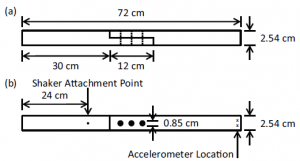
\includegraphics[width=0.5\textwidth]{./figs/300px-BRB.png}
\caption{\label{fig:org5494497}Geometry of the BRB Benchmark}
\end{figure}

A picture of the parts of the BRB is shown in Fig. \ref{fig:org5494497} and this will be used to guide the modeling here.
Standard 5/16 bolt-nut-washers will be used for the assembly. Since Bolt thread interactions won't be modeled here, the bolt shank is modeled as a smooth cylinder (see \ref{org3da75de} for more details on bolt prestress modeling).

\textbf{Note}: If you already have a model of your structure and want to just apply the node-selection/matrix extraction, you can safely ignore the sections particular to the modeling of the BRB and just go through the remaining, whose instructions are quite general.
The general principles in the modeling section are, however, recommended for all jointed structure modeling.

\subsection{A Note on Python Scripting\hfill{}\textsc{Script}}
\label{sec:orgbbb6e14}
ABAQUS Python scripting is quite powerful and will be used quite liberally throughout this tutorial. The following are some tips/tricks to get started for beginners:
\begin{itemize}
\item For beginners, the easiest way to start scripting is to open up CAE (the GUI) and do the necessary tasks. ABAQUS would have saved the actions in a Python file called \texttt{abaqus.rpy}. This is just python code that can be imported into ABAQUS to repeat the same tasks.
All standard python commands work so this makes it very helpful.
\item On Windows the \textbf{work directory} may be an unfamiliar concept (on Linux it is just the directory from which ABAQUS is launched). This directory can be manually set by \texttt{File->Set Work Directory}, following which all the files (including the \texttt{ABAQUS.rpy} file) will be put in the specified folder.
\item Fig \ref{fig:orge383030} shows a pictorial overview of the different options available in ABAQUS for scripting support. The ABAQUS PDE can be used for ABAQUS python script development.
\end{itemize}
\begin{figure}[htbp]
\centering
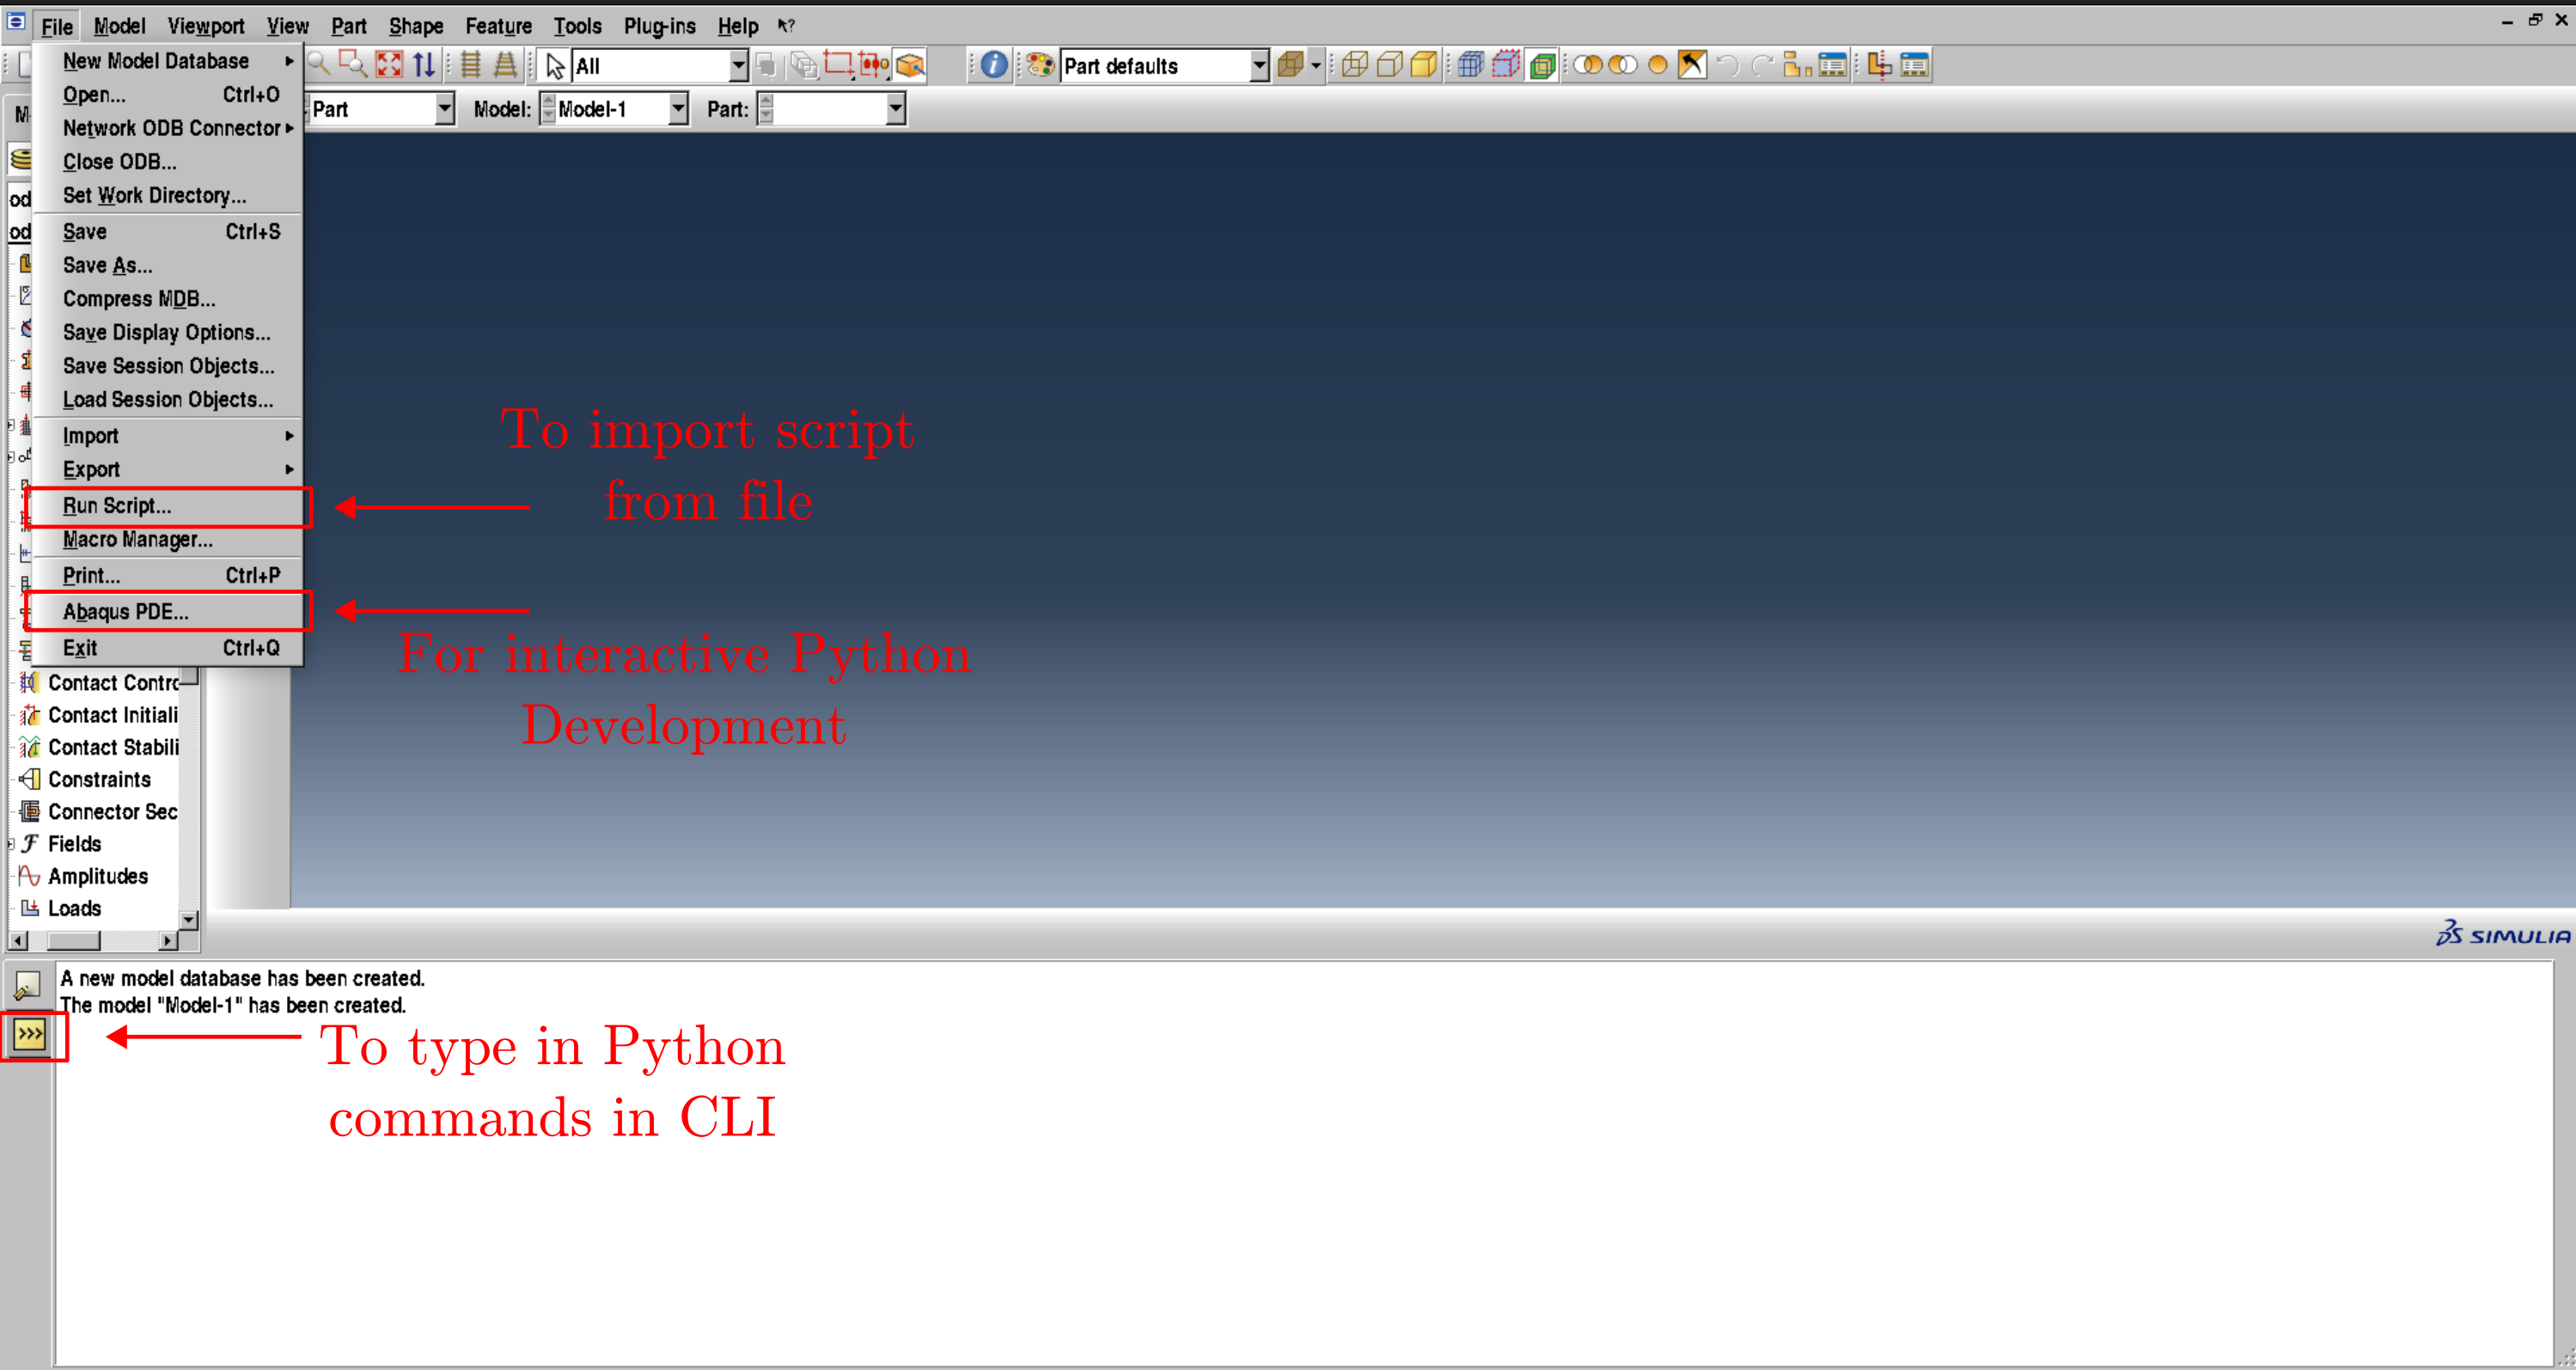
\includegraphics[width=\textwidth]{./figs/ovw.png}
\caption{\label{fig:orge383030}Options in ABAQUS for Scripting}
\end{figure}

\subsection{Modeling Parts\hfill{}\textsc{Script:GUI}}
\label{sec:org1d95fb3}
We will first model the two "halves" of the BRB. The following steps enumerate the process (can be skipped if you already have a model).

We will do the construction through ABAQUS Python code that can be imported through \texttt{File->Run Script} or just typed into the command line.

\begin{enumerate}
\item First import the following code to import all the necessary objects and then the material properties (steel, here).
\begin{verbatim}
 1  # -*- coding: utf-8 -*-
 2  import sys
 3  
 4  from part import *
 5  from material import *
 6  from section import *
 7  from assembly import *
 8  from step import *
 9  from interaction import *
10  from load import *
11  from mesh import *
12  from optimization import *
13  from job import *
14  from sketch import *
15  from visualization import *
16  from connectorBehavior import *
17  
18  mdl = mdb.models['Model-1']
19  ##############################
20  # MATERIAL PROPERTIES: STEEL #
21  ##############################
22  mdl.Material(name='STEEL')
23  
24  steel = mdl.materials['STEEL']
25  steel.Density(table=((7800.0, ), ))
26  steel.Elastic(table=((2e11, 0.29),))
27  mdl.HomogeneousSolidSection(material='STEEL', name=
28                              'Section-1', thickness=None)
\end{verbatim}
The above code creates a new material called "STEEL", with Young's Modulus 200GPa, Poisson's ratio 0.29, and density 7800 kg/m\textsuperscript{3}.
\item Now use the following to model the half beam (this can be done on CAE with the GUI quite easily).
\begin{verbatim}
 29  mdl = mdb.models['Model-1']
 30  
 31  ###################
 32  # PART : HALFBEAM #
 33  ###################
 34  # 1. Sketch and Extrude
 35  mdl.ConstrainedSketch(name='__profile__', sheetSize=2.0)
 36  sktch = mdl.sketches['__profile__']
 37  sktch.Line(point1=(-36e-2, 1.27e-2), point2=(-6e-2, 1.27e-2))
 38  sktch.Line(point1=(-6e-2, 1.27e-2), point2=(-6e-2, 0))
 39  sktch.Line(point1=(-6e-2, 0), point2=(6e-2,0))
 40  sktch.Line(point1=(6e-2,0), point2=(6e-2,-1.27e-2))
 41  sktch.Line(point1=(6e-2,-1.27e-2), point2=(-36e-2,-1.27e-2))
 42  sktch.Line(point1=(-36e-2,-1.27e-2), point2=(-36e-2,1.27e-2))
 43  
 44  mdl.Part(dimensionality=THREE_D, name='HALFBEAM', type=DEFORMABLE_BODY)
 45  hfbm = mdl.parts['HALFBEAM']
 46  hfbm.BaseSolidExtrude(depth=25.4e-3, sketch=sktch)
 47  del sktch
 48  
 49  # 2. Cut out Holes
 50  mdl.ConstrainedSketch(name='__profile__', sheetSize=2.0,
 51                        transform=
 52                        hfbm.MakeSketchTransform(
 53                            sketchPlane=hfbm.faces[2],
 54                            sketchPlaneSide=SIDE1,
 55                            sketchUpEdge=hfbm.edges[8],
 56                            sketchOrientation=RIGHT,
 57                            origin=(0.0, 0.0, 1.27e-2)))
 58  sktch = mdl.sketches['__profile__']
 59  cs = [-3e-2, 0.0, 3e-2];
 60  gs = []
 61  for i in range(3):
 62      gs.append(sktch.CircleByCenterPerimeter(center=(cs[i], 0),
 63                                              point1=(cs[i]+0.85e-2/2, 0)))
 64  
 65  hfbm.CutExtrude(sketchPlane=hfbm.faces[2], sketchPlaneSide=SIDE1,
 66                  sketchUpEdge=hfbm.edges[8],
 67                  sketchOrientation=RIGHT, sketch=sktch)
 68  
 69  
 70  # 3. Partition object
 71  hfbm.PartitionCellByExtendFace(cells=hfbm.cells,
 72                                 extendFace=hfbm.faces[6])
 73  hfbm.PartitionCellByExtendFace(cells=hfbm.cells,
 74                                 extendFace=hfbm.faces[7])
 75  
 76  mdl.ConstrainedSketch(name='__profile__', sheetSize=2.0,
 77                        gridSpacing=30e-3, transform=
 78                        hfbm.MakeSketchTransform(
 79                            sketchPlane=hfbm.faces[11],
 80                            sketchPlaneSide=SIDE1,
 81                            sketchUpEdge=hfbm.edges[27],
 82                            sketchOrientation=RIGHT,
 83                            origin=(0.0, 0.0, 1.27e-2)))
 84  sktch = mdl.sketches['__profile__']
 85  cs = [-3e-2, 0.0, 3e-2];
 86  wor = i2m*0.34375
 87  for i in range(3):
 88      sktch.CircleByCenterPerimeter(center=(cs[i], 0),
 89                                    point1=(cs[i]+wor, 0))
 90  hfbm.PartitionCellBySketch(cells=hfbm.cells, sketch=sktch,
 91                             sketchUpEdge=hfbm.edges[27],
 92                             sketchPlane=hfbm.faces[11])
 93  hfbm.PartitionCellByExtrudeEdge(cells=hfbm.cells, edges=hfbm.edges[0],
 94                                  line=hfbm.edges[-1], sense=FORWARD)
 95  hfbm.PartitionCellByExtrudeEdge(cells=hfbm.cells, edges=hfbm.edges[3],
 96                                  line=hfbm.edges[-1], sense=FORWARD)
 97  hfbm.PartitionCellByExtrudeEdge(cells=hfbm.cells, edges=hfbm.edges[6],
 98                                  line=hfbm.edges[-1], sense=FORWARD)
 99  
100  pt = hfbm.InterestingPoint(edge=hfbm.edges[-2], rule=MIDDLE)
101  hfbm.PartitionCellByPlanePointNormal(cells=hfbm.cells, point=pt,
102                                       normal=hfbm.edges[-2])
103  
104  pt = hfbm.InterestingPoint(edge=hfbm.edges[75], rule=MIDDLE)
105  hfbm.PartitionCellByPlanePointNormal(cells=hfbm.cells, point=pt,
106                                       normal=hfbm.edges[75])
107  
108  pt = hfbm.InterestingPoint(edge=hfbm.edges[39], rule=MIDDLE)
109  hfbm.PartitionCellByPlanePointNormal(cells=hfbm.cells, point=pt,
110                                       normal=hfbm.edges[39])
111  
112  pt = hfbm.InterestingPoint(edge=hfbm.edges[85], rule=MIDDLE)
113  hfbm.PartitionCellByPlanePointNormal(cells=hfbm.cells, point=pt,
114                                       normal=hfbm.edges[85])
115  
116  pt = hfbm.InterestingPoint(edge=hfbm.edges[39], rule=MIDDLE)
117  hfbm.PartitionCellByPlanePointNormal(cells=hfbm.cells, point=pt,
118                                       normal=hfbm.edges[39])
119  
120  pt = hfbm.InterestingPoint(edge=hfbm.edges[41], rule=MIDDLE)
121  hfbm.PartitionCellByPlanePointNormal(cells=hfbm.cells, point=pt,
122                                       normal=hfbm.edges[41])
123  
124  pt = hfbm.InterestingPoint(edge=hfbm.edges[111], rule=MIDDLE)
125  hfbm.PartitionCellByPlanePointNormal(cells=hfbm.cells, point=pt,
126                                       normal=hfbm.edges[111])
127  
128  pt = hfbm.InterestingPoint(edge=hfbm.edges[135], rule=MIDDLE)
129  hfbm.PartitionCellByPlanePointNormal(cells=hfbm.cells, point=pt,
130                                       normal=hfbm.edges[135])
131  
132  # 4. Assign Material
133  regn = hfbm.Set(cells=hfbm.cells, name='Set-1')
134  hfbm.SectionAssignment(region=regn, sectionName='Section-1')
\end{verbatim}
\end{enumerate}
\definecolor{osbe-bg}{HTML}{cccccc}\colorlet{osbe-fg}{black}\begin{quote}
                              \begin{tcolorbox}[colback=osbe-bg,colframe=osbe-fg,title={Scripting note},sharp corners,boxrule=0.4pt]
You can see that certain faces and edges were used in the above.
A quick way to check which face is what will be to use the \texttt{highlight} command on the ABAQUS python console.
Here is an example:
\begin{center}
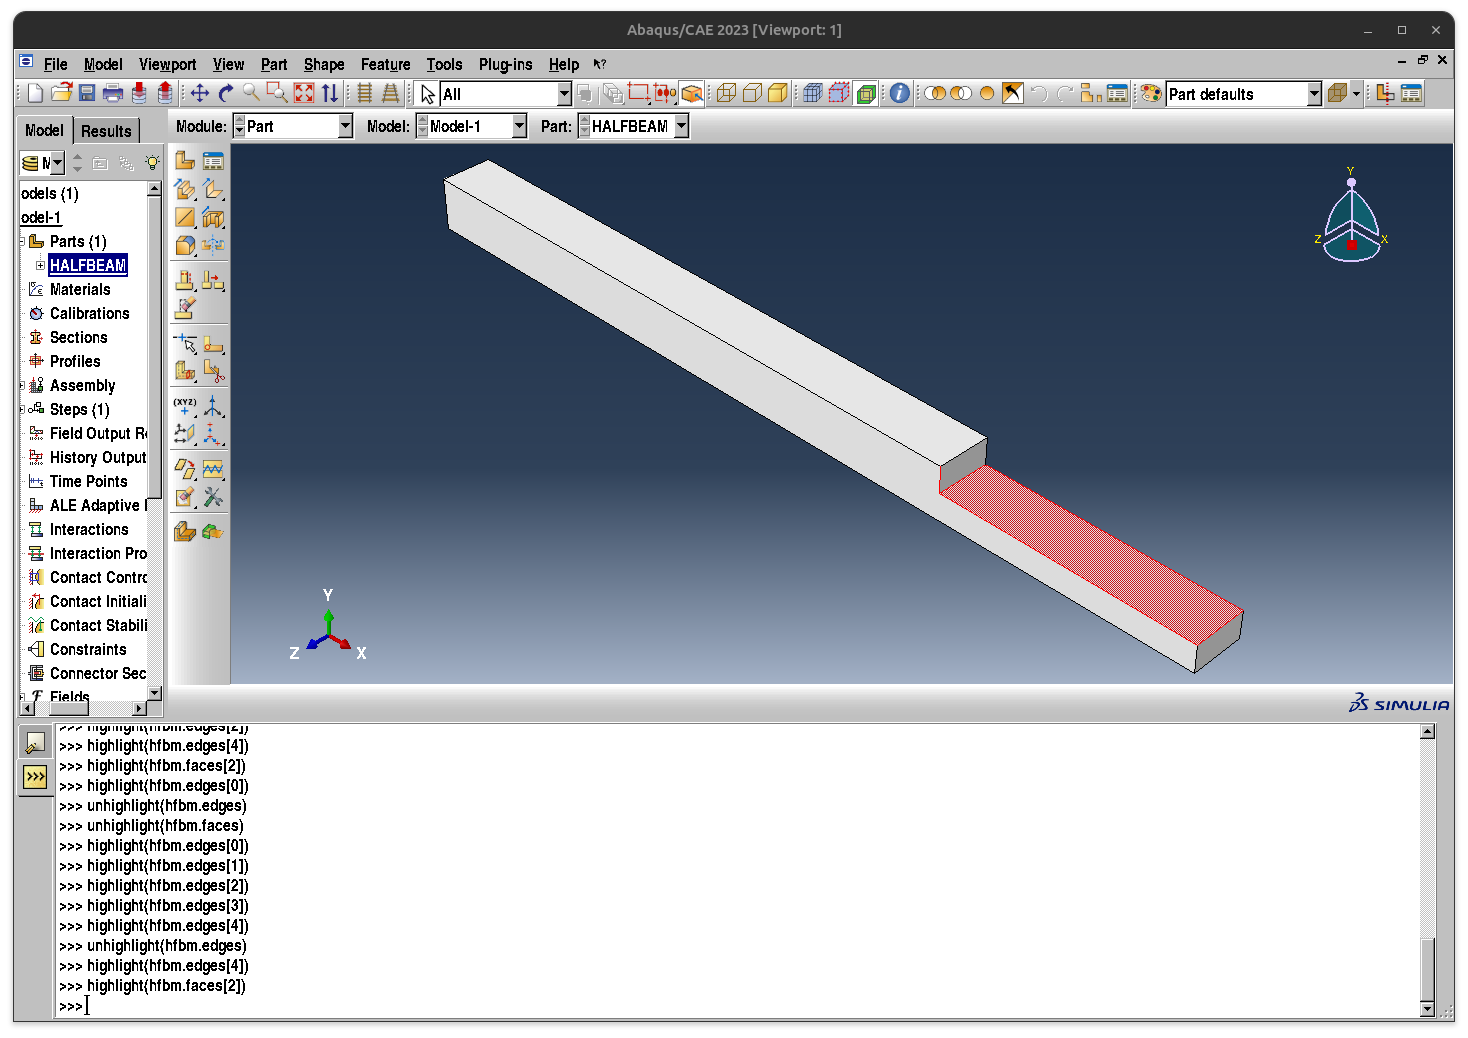
\includegraphics[width=.9\linewidth]{./figs/highl.png}
\end{center}


               \end{tcolorbox}
\end{quote}
At the end of this step, you should have a partitioned part that looks like this.
The partitioning is done in this way to help with the seeded meshing, constraint enforcement, etc.
\begin{center}
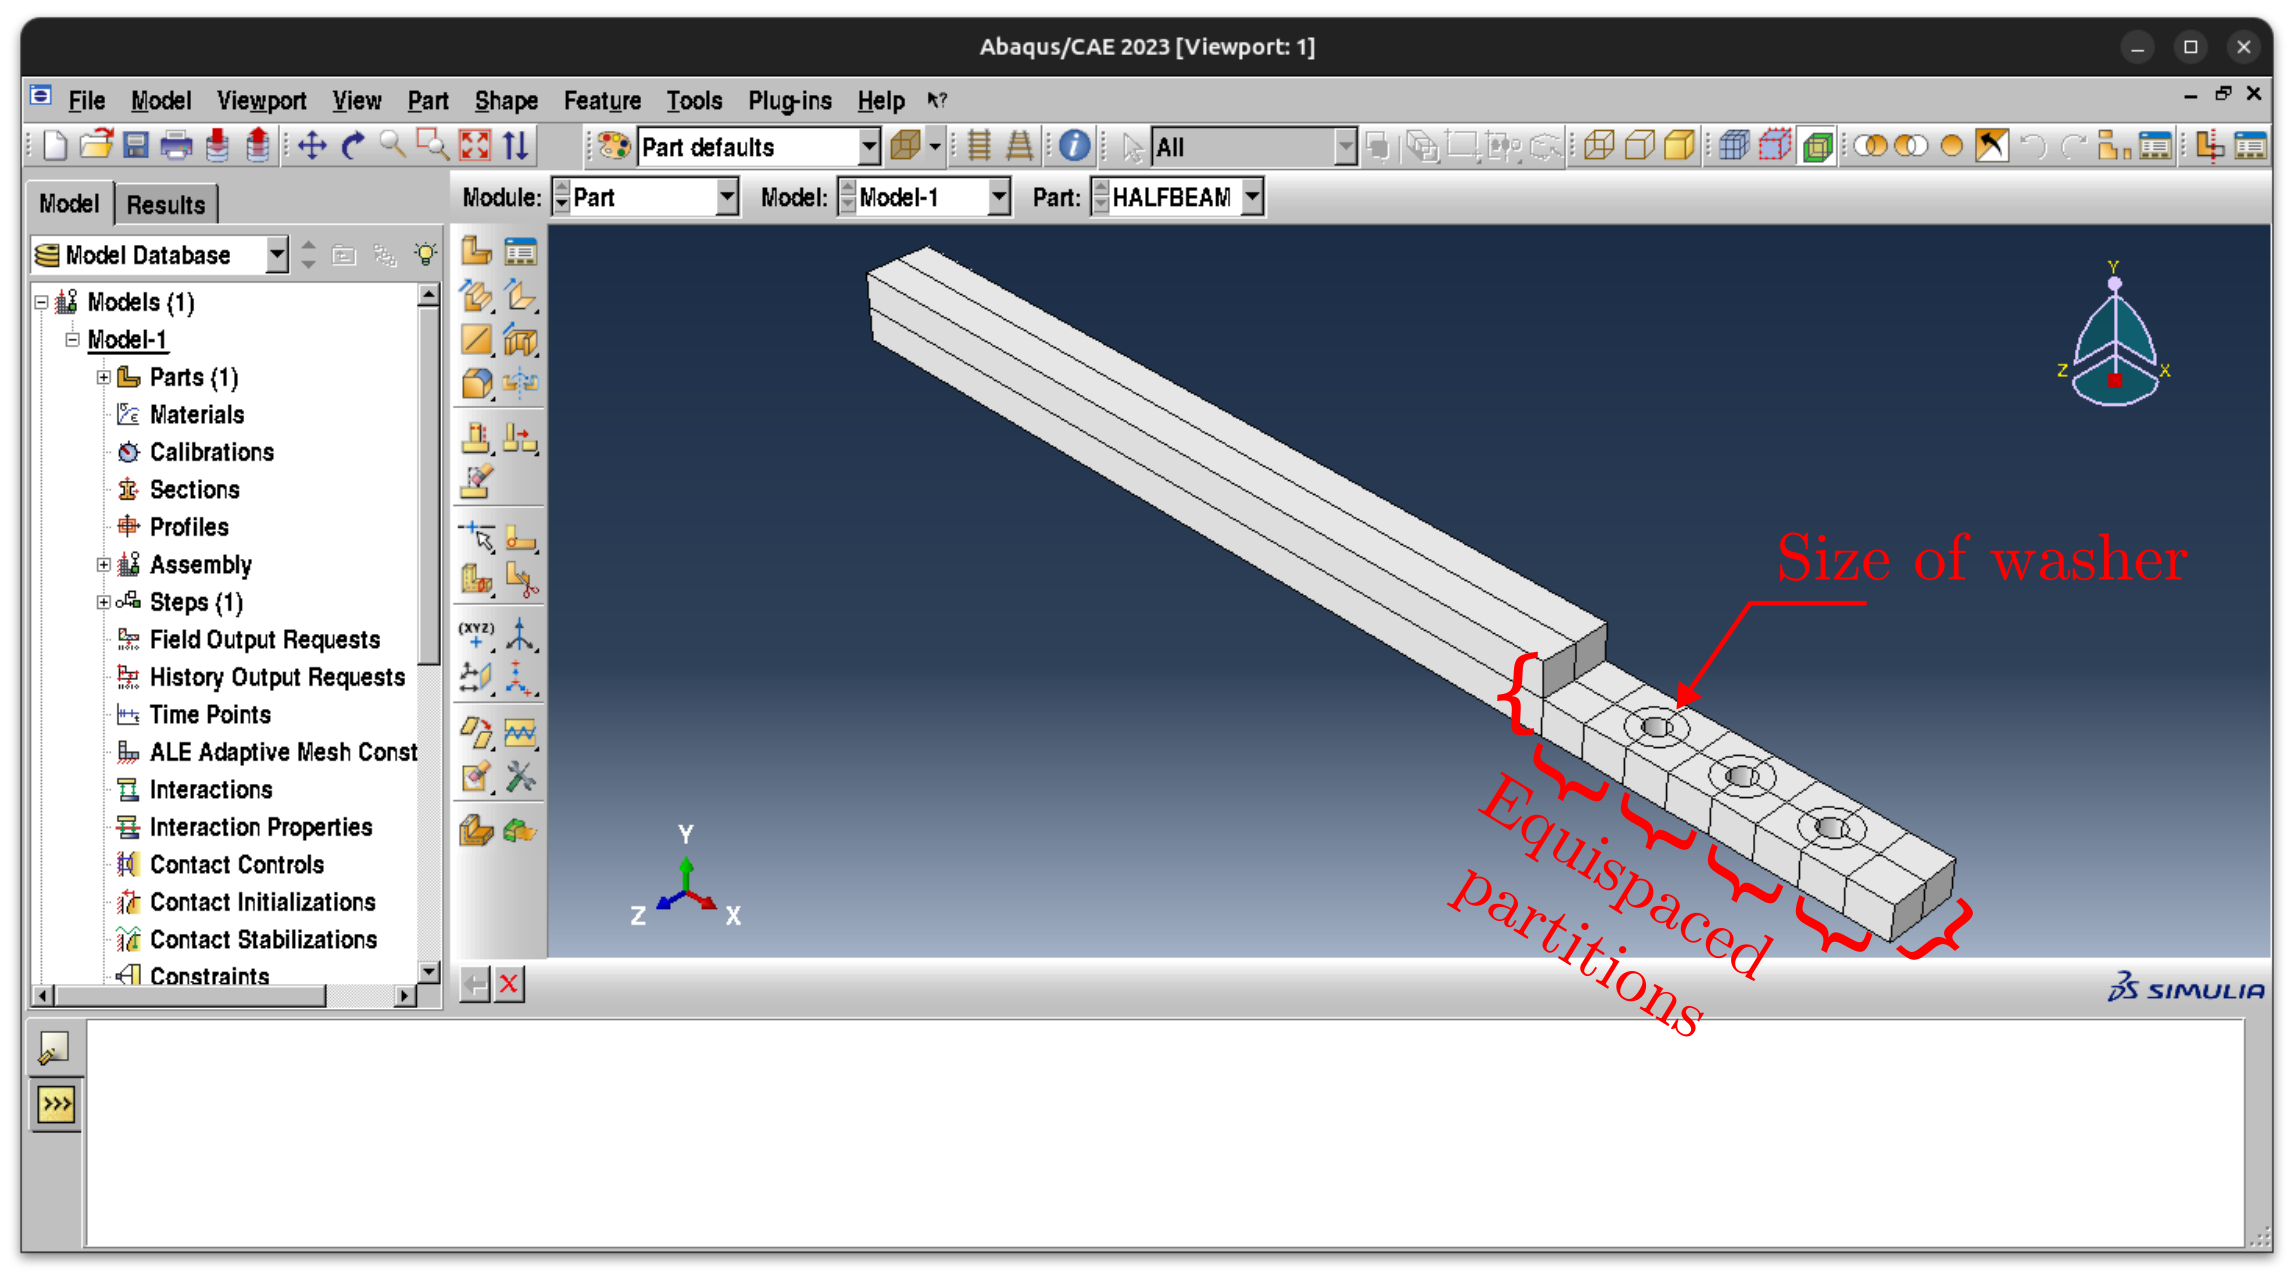
\includegraphics[width=.9\linewidth]{./figs/parthb.png}
\end{center}
\definecolor{osbe-bg}{HTML}{cccccc}\colorlet{osbe-fg}{black}\begin{quote}
                              \begin{tcolorbox}[colback=osbe-bg,colframe=osbe-fg,title={IMPORTANT! Geometry Correction Note},sharp corners,boxrule=0.4pt]
You have to ensure that the curved edges on the above are, indeed, single edges. You will run into meshing issues if this is not the case.
If not, you will have to use the "Merge Edges" tool in the Part module and individually select each edge and merge them.
\begin{center}
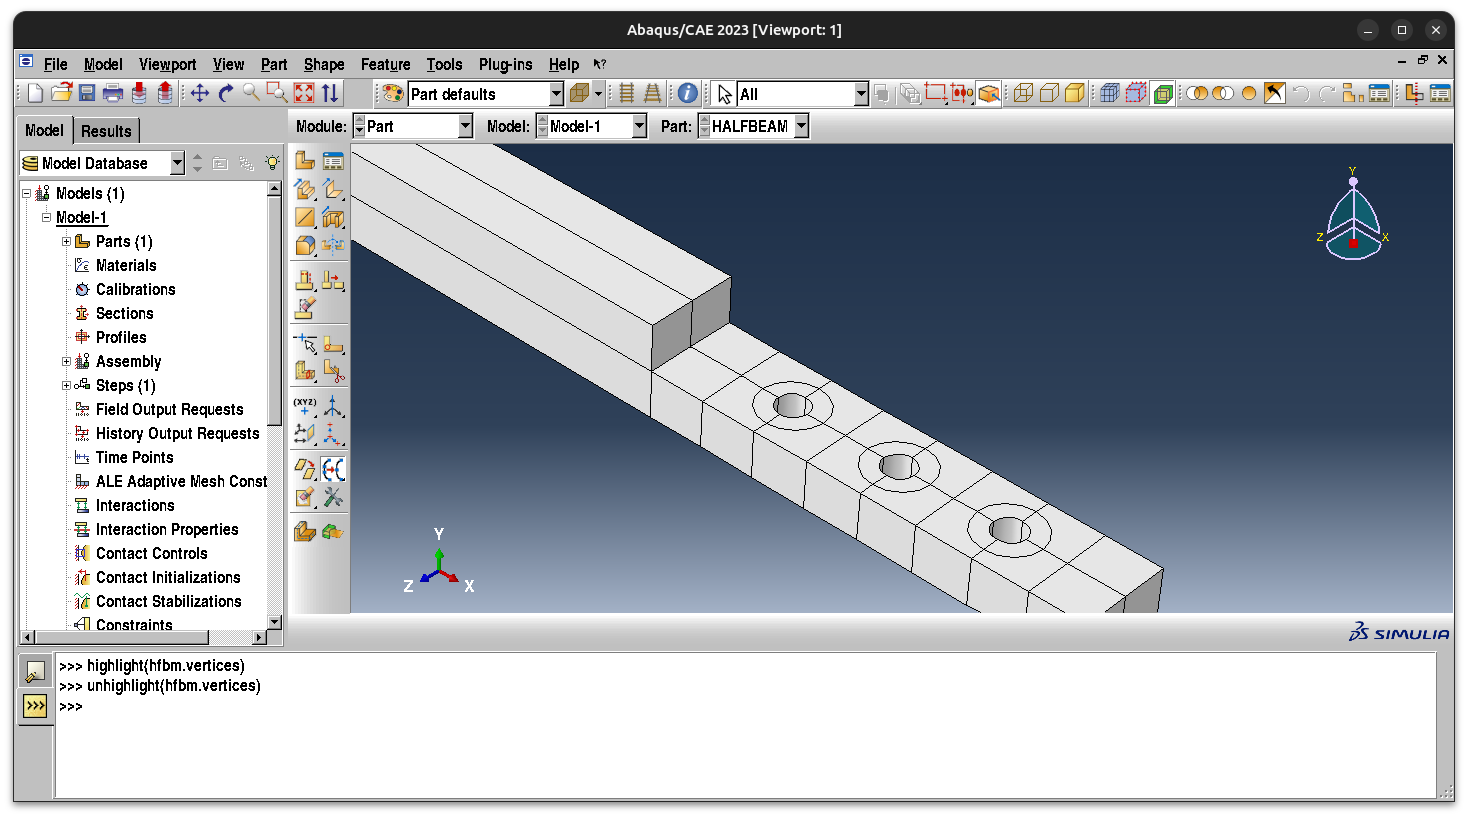
\includegraphics[width=.9\linewidth]{./figs/medg.png}
\end{center}


               \end{tcolorbox}
\end{quote}
\begin{enumerate}
\item Create a Reference Point Part called \texttt{REFPT}.
This will be necessary for the application of bolt prestress (see \ref{org3da75de} below).
\begin{verbatim}
135  rpt = mdl.Part(name='REFPT', dimensionality=THREE_D, 
136                 type=DEFORMABLE_BODY)
137  rpt.ReferencePoint(point=(0.0, 0.0, 0.0))
138  
139  rpt.Set(name='Set-1', referencePoints=rpt.referencePoints.values())
\end{verbatim}
\item Now import the nuts, washers and bolts by importing the file \url{https://github.com/Nidish96/Abaqus4Joints/blob/main/scripts/c\_nutwasherbolt\_516.py}.
You should be able to see the nut, washer and bolt, along with the half beam and reference point created before, as follows after importing:
\begin{center}
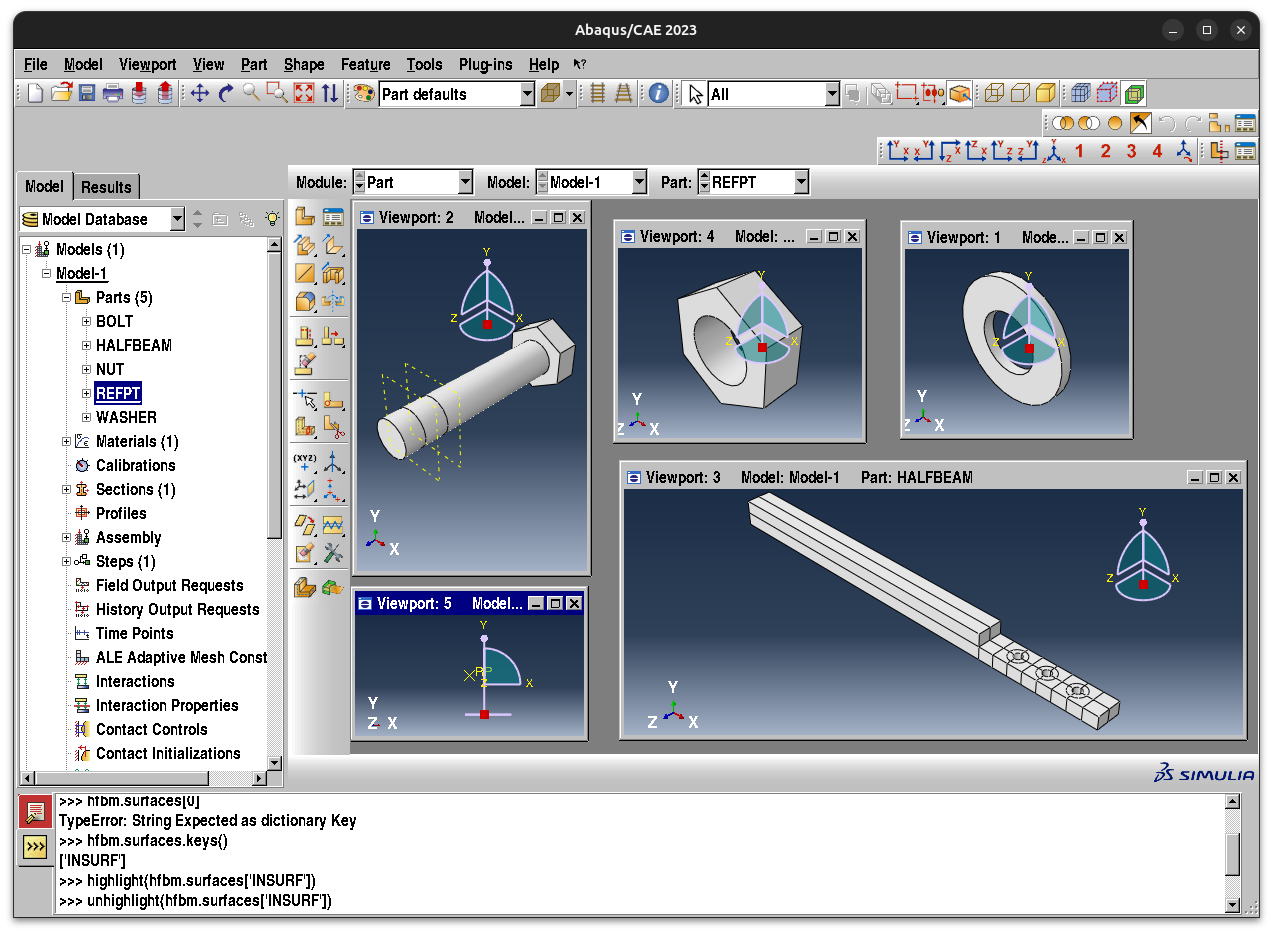
\includegraphics[width=.9\linewidth]{./figs/nwb.png}
\end{center}
The Python script also assigns the material "STEEL" (see above) to the parts.
\end{enumerate}

The file \href{https://github.com/Nidish96/Abaqus4Joints/blob/main/assets/assembly/model\_step0.cae}{model\_step0.cae} stores the CAE file at the end of the above steps (building parts, and partitioning).
\subsection{Creating appropriate surface sets\hfill{}\textsc{GUI}}
\label{sec:org64c9343}
It is necessary to choose appropriate surface sets for the constraint enforcement and, eventually, the interfacial mesh extraction.
Doing this with surfaces (before meshing) is advantageous since the same scripts can be reused even if the model is remeshed.
\begin{enumerate}
\item First select the \textbf{interfacial faces} on the half beam model and assign the name \texttt{INSURF} to it.
You can do this through \texttt{Tools->Surface->Create} and then selecting the appropriate faces through the GUI.
Select the faces by holding \texttt{Shift} and deselect by holding \texttt{Ctrl}.
Here is a picture of the surface highlighted in the viewport.
\begin{center}
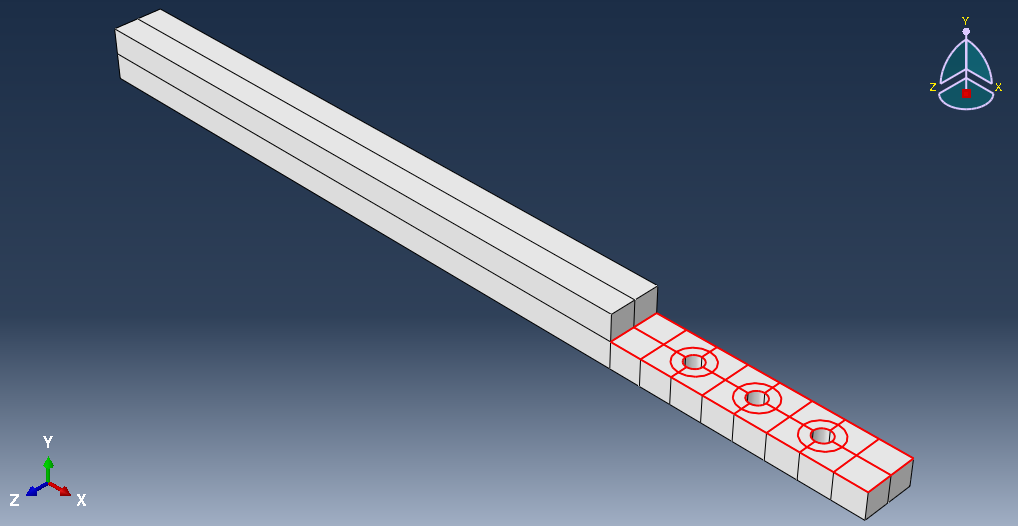
\includegraphics[width=0.5\textwidth]{./figs/insurf.png}
\end{center}
\item Turn to the \emph{outside} of the beam and select the faces around the bolts individually and name them \texttt{BmW1}, \texttt{BmW2}, and \texttt{BmW3} respectively.
These will be tied to the washer for the analysis. (\texttt{BmWi} denotes the i\textsuperscript{th} Beam-Washer contact).
Here is a picture of the relevant surfaces highlighted (using different colors for each).
\begin{center}
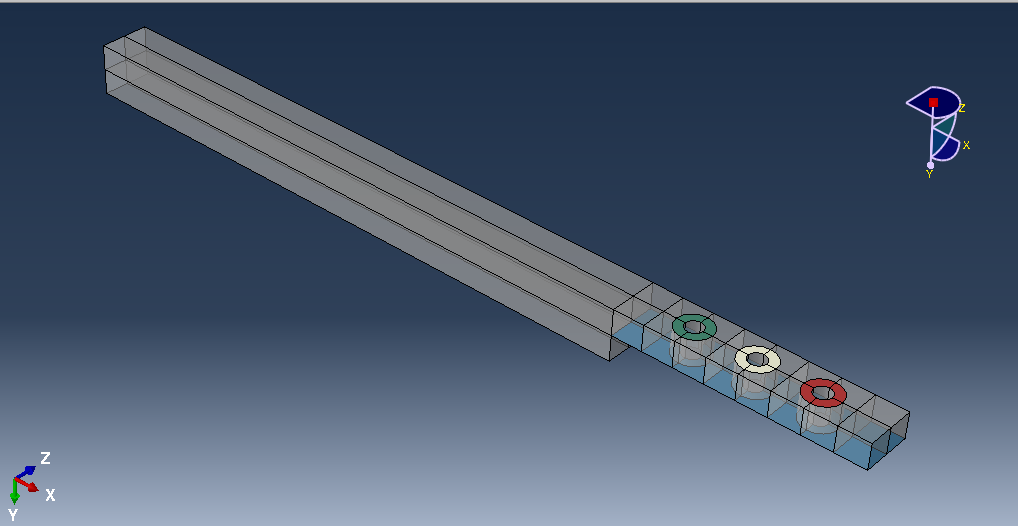
\includegraphics[width=0.5\textwidth]{./figs/bmwsurfs.png}
\end{center}
\item Create two surfaces on the \texttt{BOLT} model as shown in the figure below.
Name the surface marked white as \texttt{BlW} and the surface marked green as \texttt{BN}.
(\texttt{BlW} denotes the Bolt-Washer contact surface; \texttt{BN} denotes the Bolt-Nut contact surface)
\begin{center}
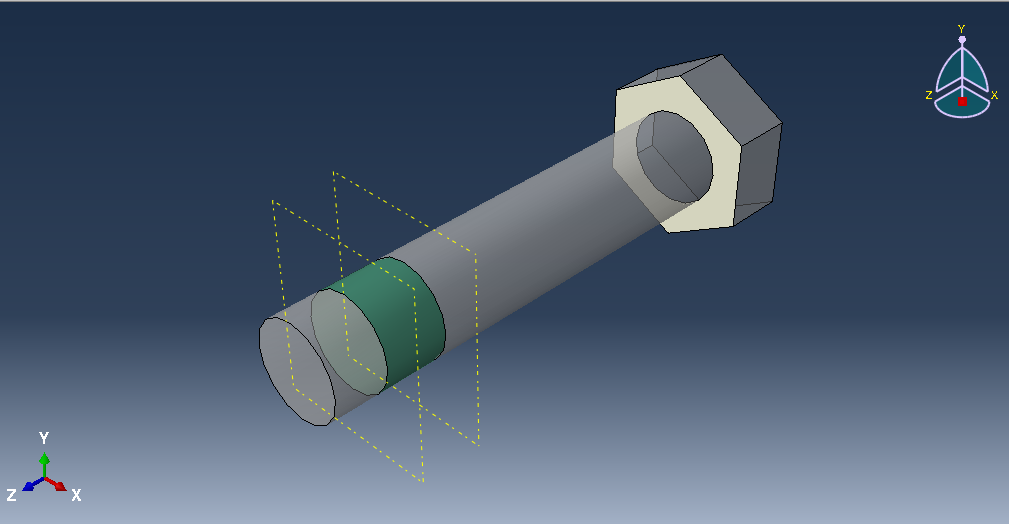
\includegraphics[width=0.4\textwidth]{./figs/boltsurfs.png}
\end{center}
\item Create two surfaces on the \texttt{NUT} model as shown in the figure below.
Name the white surface as \texttt{NW} and the green surface as \texttt{NB}.
(\texttt{NW} denotes the Nut-Washer contact surface; \texttt{NB} denotes the Nut-Bolt contact surface)
\textbf{Note the direction axes carefully.}
\begin{center}
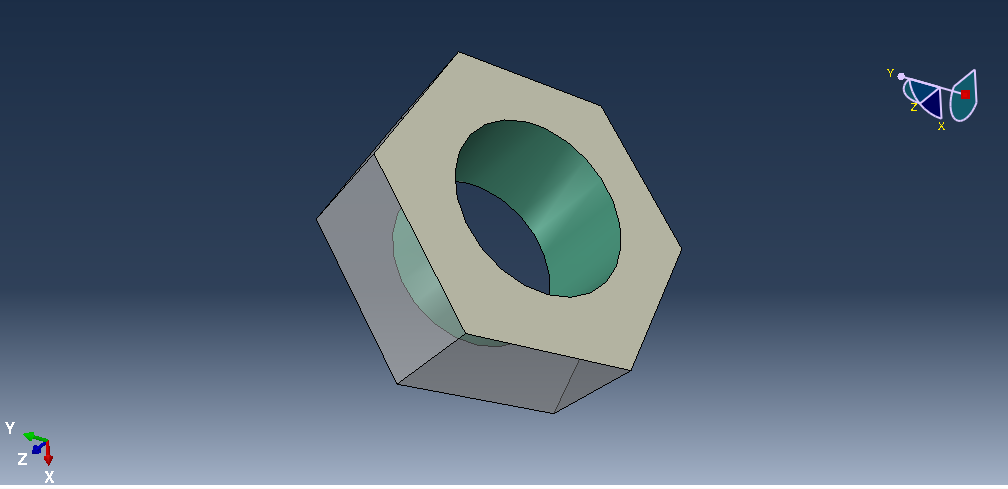
\includegraphics[width=0.4\textwidth]{./figs/nutsurfs.png}
\end{center}
\item Create two surface on the \texttt{WASHER} model and label them as \texttt{WSTOP} and \texttt{WSBOT} (short for Washer-Surface Top and Bottom).
Here is a graphical depiction of the model with the surfaces.
\begin{center}
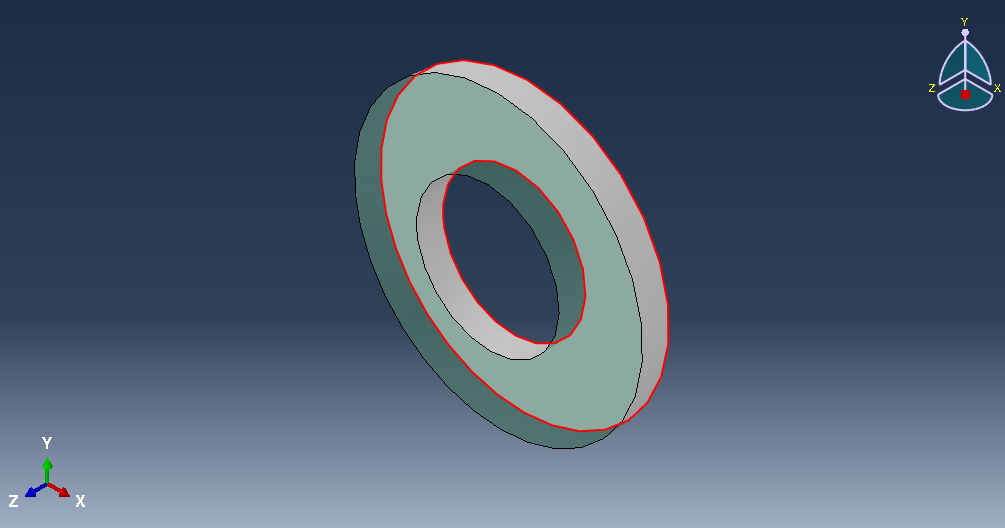
\includegraphics[width=0.4\textwidth]{./figs/wshrsurf.png}
\end{center}
\end{enumerate}

Now all the parts have been created and relevant surfaces have been identified.
\textbf{Note}: It is important to have traceable but short names so that a lot of the repetitive tasks can be sped up considerably using scripting.
\subsection{Create Assembly\hfill{}\textsc{GUI}}
\label{sec:org8a187c8}
\textbf{Note}: While importing the parts, choose Instance Type as "Independent (Mesh on Instance)".
This will be advantageous if we want to modify the meshes just at the interface for mirror symmetry.
We will do independent meshing since it is good practice, although independent meshes are not a requirement for this example (dependent meshes can be used due to symmetry).

\begin{enumerate}
\item Import the two beams and re-orient/move them as follows.
\textbf{Note that the bolt-axis has to be pointed in the +z direction.}
This will be the convention followed throughout this tutorial.
The green beam in the following is renamed as \texttt{TOPBEAM} and the white beam in the following is renamed as \texttt{BOTBEAM}.
\begin{center}
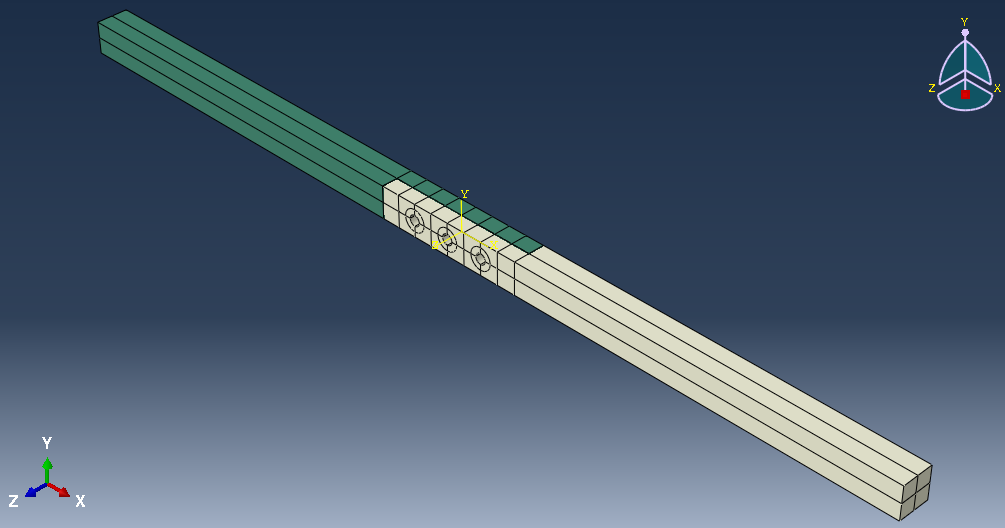
\includegraphics[width=0.55\textwidth]{./figs/asb1.png}
\end{center}
\item Import one instance each of the \texttt{BOLT} and \texttt{NUT} and 2 instances of the \texttt{WASHER} and assemble them as shown.
Ensure that the washer is oriented (on each side) with the \texttt{WSTOP} oriented in the \texttt{-z} direction and the \texttt{WSBOT} is oriented in the \texttt{+z} direction.
Rename the washer instances in the top and bottom as \texttt{TOPWASHER-1} and \texttt{BOTWASHER-1} respectively.
Rename the bolt and nut as \texttt{NUT-1} and \texttt{BOLT-1} respectively.
\begin{center}
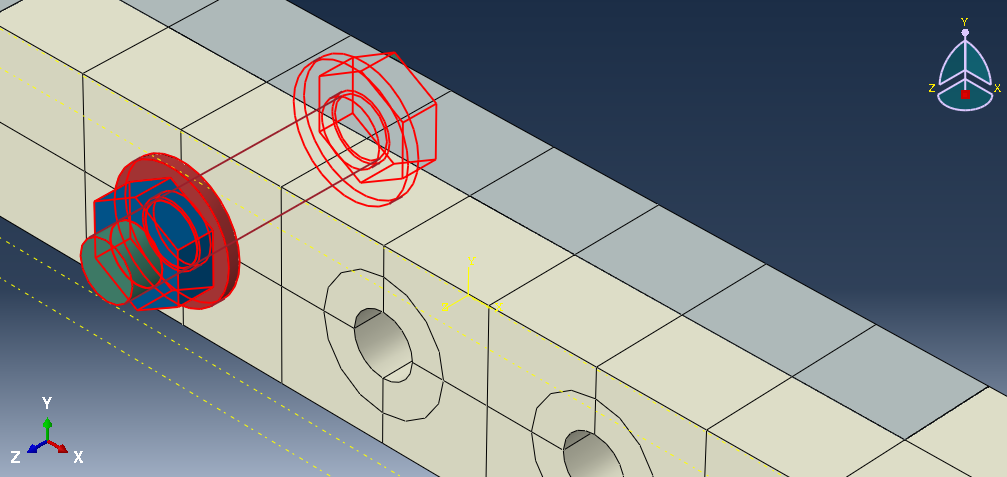
\includegraphics[width=0.5\textwidth]{./figs/asbwn.png}
\end{center}
\item Import one instance of the reference point \texttt{REFPT}.
As mentioned before, this will be used to enforce bolt prestress.
This will be achieved by first placing it at the centroid of the intersection of the \texttt{BOLT} and \texttt{NUT} (surfaces \texttt{BN} and \texttt{NB}).
It is important that the reference point is placed at the centroid.
This can be done in the GUI by first moving it to an external point and then translating it along the axis.
The figure below shows an example (a datum point was used for this here).
Rename this to \texttt{BPT-1} (standing for Bolt Point 1).
\begin{center}
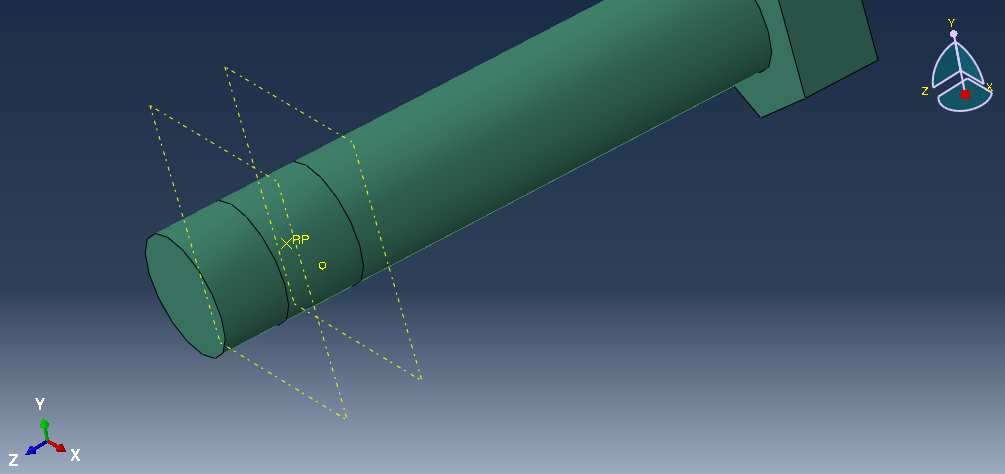
\includegraphics[width=0.55\textwidth]{./figs/asrpt.png}
\end{center}
\item Now import another instance of the reference point \texttt{REFPT} and translate it to be coincident with \texttt{BPT-1}.
Rename this \texttt{NPT-1} (standing for Nut Point 1).
These two points will have to be on the same geometrical point but equal and opposite forces will be applied for the force application (see \ref{org3da75de} below for those steps).
The point \texttt{BPT-1} will be coupled to the bolt surface \texttt{BN} and \texttt{NPT-1} will be tied to the nut surface \texttt{NB} through RBE3 elements.
\item Use the "Linear Pattern" dialog and copy the bolt-washer-washer-nut assembly thrice along the beam such that the assembly is complete.
The figure below shows the final assembly along with a representation of the names of the different parts.
Recall that  the beam shown in the figure below is \texttt{TOPBEAM} and the hidden one is \texttt{BOTBEAM}.
\begin{center}
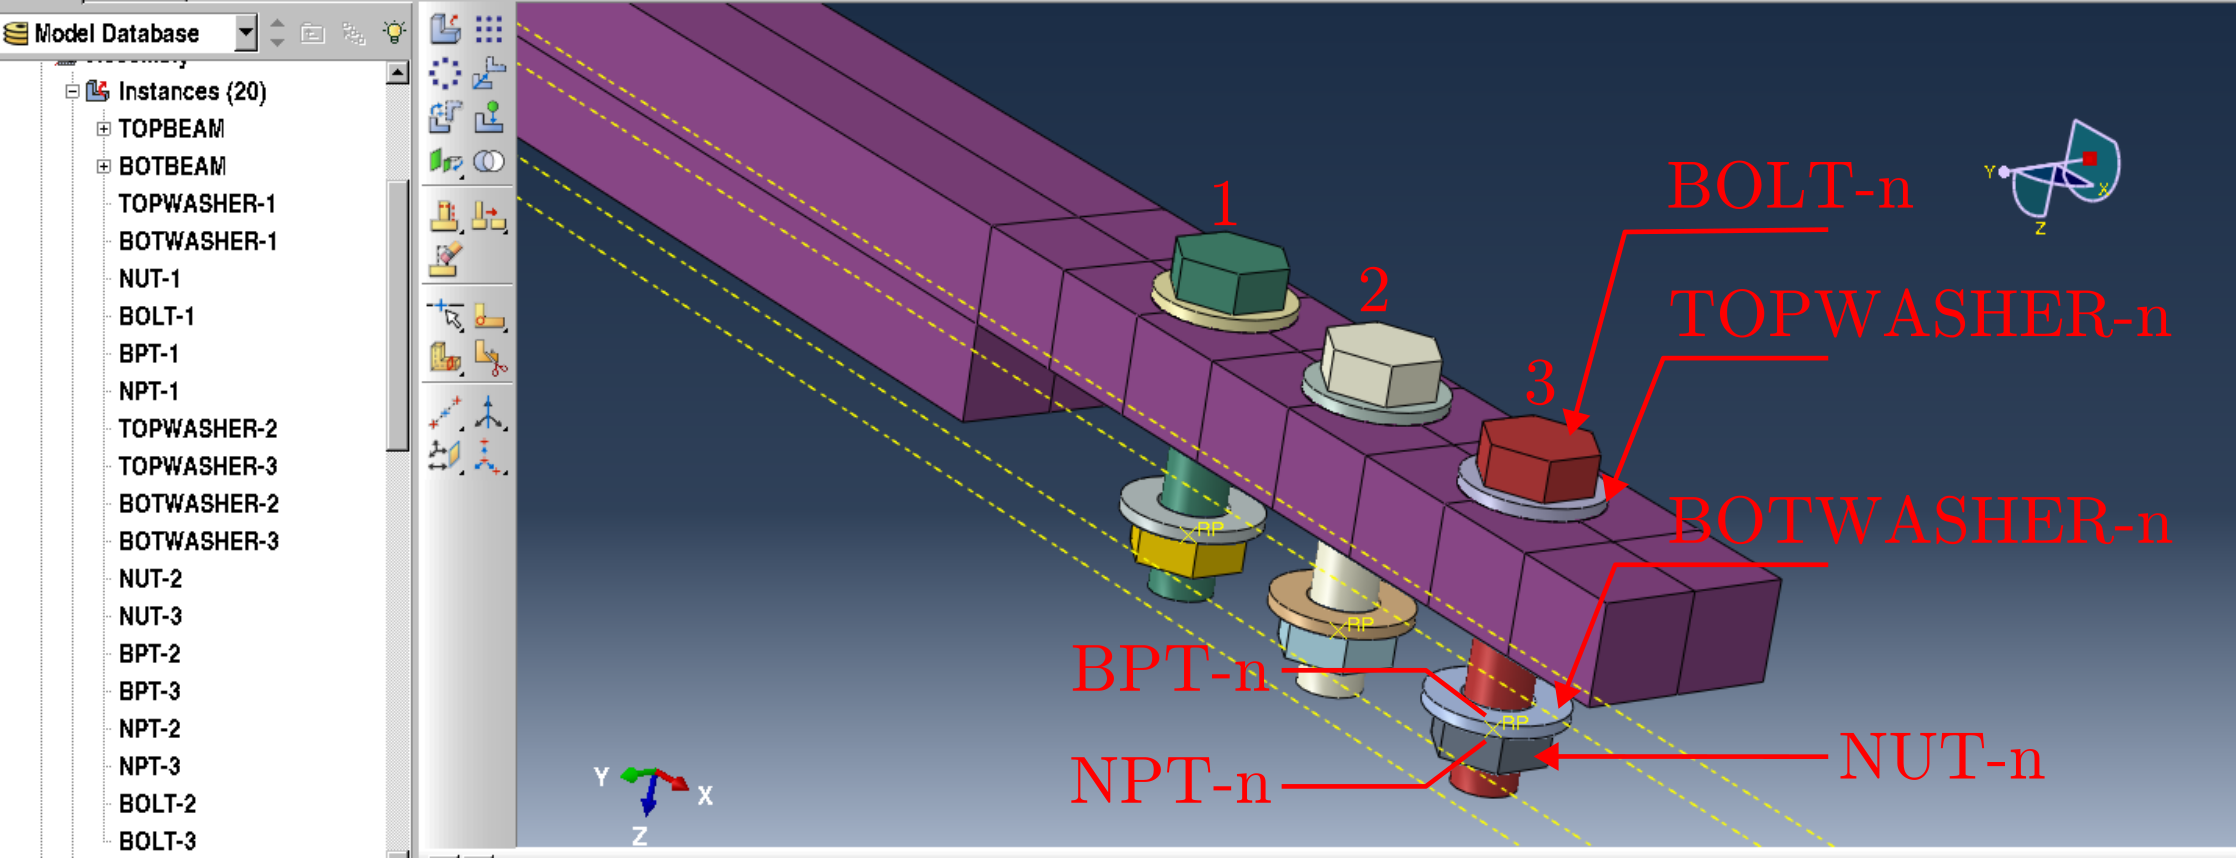
\includegraphics[width=.9\linewidth]{./figs/as3bwn.png}
\end{center}
\end{enumerate}

Now that the assembly is complete, the relevant constraints will have to be enforced, followed by a realization of the bolt preload.
\section{Constraints}
\label{sec:org9d8abcf}
\subsection{Tie-Constraint Enforcement\hfill{}\textsc{Script:GUI}}
\label{sec:org21b1024}
All the following operations can be conducted in the \texttt{Interaction} module in CAE.
But since selecting each surface can be a time-consuming process, we use the following for-loop in ABAQUS-python (either call it as a script or just copy paste it into the CLI) to make the required tie constraints.
Specifically, it ties the Bolt-Washer, Nut-Washer, and Washer-Beam surfaces.
Note that in the last set of constraints, we recall the fact that the bottom beam is flipped.
So \texttt{WASHER-1} is tied to \texttt{BmW3} of the bottom beam (and so on for 2,3).
\begin{verbatim}
 1  mdl = mdb.models['Model-1']
 2  ras = mdl.rootAssembly
 3  
 4  for i in range(1, 4):
 5      # Bolt-Washer Constraints
 6      mdl.Tie(name='BW-%d' %(i),
 7              main=ras.instances['TOPWASHER-%d' %(i)].surfaces['WSTOP'],
 8              secondary=ras.instances['BOLT-%d' %(i)].surfaces['BlW'],
 9              positionToleranceMethod=COMPUTED, adjust=ON,
10              tieRotations=ON, thickness=ON)
11  
12      # Nut-Washer Constraints
13      mdl.Tie(name='NW-%d' %(i),
14              main=ras.instances['BOTWASHER-%d' %(i)].surfaces['WSBOT'],
15              secondary=ras.instances['NUT-%d' %(i)].surfaces['NW'],
16              positionToleranceMethod=COMPUTED, adjust=ON,
17              tieRotations=ON, thickness=ON)
18  
19      # TopWasher-Beam Constraints
20      mdl.Tie(name='BmTW-%d' %(i),
21              main=ras.instances['TOPBEAM'].surfaces['BmW%d' %(i)],
22              secondary=ras.instances['TOPWASHER-%d' %(i)].surfaces['WSBOT'],
23              positionToleranceMethod=COMPUTED, adjust=ON,
24              tieRotations=ON, thickness=ON)
25  
26      # BotWasher-Beam Constraints
27      mdl.Tie(name='BmBW-%d' %(i),
28              main=ras.instances['BOTBEAM'].surfaces['BmW%d' %((3-i)%3+1)],
29              secondary=ras.instances['BOTWASHER-%d' %(i)].surfaces['WSTOP'],
30              positionToleranceMethod=COMPUTED, adjust=ON,
31              tieRotations=ON, thickness=ON)
\end{verbatim}
\subsection{Bolt Preload Realization\hfill{}\textsc{Script:GUI}}
\label{sec:org5423265}
\label{org3da75de}
You might already have encountered the different parts of the model above that were carefully constructed for the bolt preload application (bolt-shank partitioning, reference points, etc.).
\definecolor{osbe-bg}{HTML}{cccccc}\colorlet{osbe-fg}{black}\begin{quote}
                              \begin{tcolorbox}[colback=osbe-bg,colframe=osbe-fg,title={What 's wrong with the inbuilt Bolt Pretension in ABAQUS?},sharp corners,boxrule=0.4pt]
\textbf{The ABAQUS Approach}
\begin{itemize}
\item You can find the ABAQUS documentation for the bolt load \href{https://classes.engineering.wustl.edu/2009/spring/mase5513/abaqus/docs/v6.6/books/usi/default.htm?startat=pt04ch21s02s01.html}{here}.
\item ABAQUS/CAE applies bolt load by specifying a \textbf{bolt cross-section}, a \textbf{bolt axis}, and the \textbf{bolt load}.
\item The documentation for the ABAQUS implementation can be found \href{https://classes.engineering.wustl.edu/2009/spring/mase5513/abaqus/docs/v6.6/books/usb/default.htm?startat=pt07ch27s05aus102.html\#usb-prc-ppretension}{here}.
\item The load is applied in the context of a constraint:
\begin{itemize}
\item It can be a load constraint wherein the displacements/strains at the cross-section are adjusted to match the load.
\item It can be a deformation constraint, wherein the loads are adjusted.
\end{itemize}
\item In either case, the bolt load \textbf{can not be written down as a constant load vector} that can be exported/used elsewhere.
\item It is therefore not possible to use the inbuilt bolt pretension in a substructured analysis, for example.
\item Here are the \href{https://classes.engineering.wustl.edu/2009/spring/mase5513/abaqus/docs/v6.6/books/usb/default.htm?startat=pt07ch27s05aus102.html\#usb-prc-ppretension}{documented limitations}:
\begin{itemize}
\item An assembly load cannot be specified within a substructure.
\item If a submodeling analysis is performed, any pre-tension section should not cross regions where driven nodes are specified.
\item Nodes of a pre-tension section should not be connected to other parts of the body through multi-point constraints.
\end{itemize}
\end{itemize}

\textbf{Our Approach}
\begin{itemize}
\item Our method of bolt pretension application addresses all the above issues pertaining to substructuring/submodeling by using \textbf{Distributed Coupling} elements (aka RBE3/Spider elements in other FE software).
\item We will first couple the bolt-shank area that is in contact with the nut (the thread area) to a 6DOF point (3 translations + 3 rotations), and do the same for the nut inner surface, with another point, using \textbf{Distributed coupling} elements.
\item The bolt and nut will be "fastened" by arresting every DOF in these two nodes except the axial DOF. This will ensure that the only relative displacement between the bolt and nut are axial, which may result from tightening/loosening of the bolt.
\item A \textbf{"pulling force" is applied on the bolt-coupling node}, which acts as the tension on the bolt, and a \textbf{"pushing force" is applied on the nut-coupling node}, which acts to maintain the system's equilibrium, i.e., fastening.
\item It is understood that there is an interface that the assembly is tightening, which should provide the required reaction forces to balance everything out.
\item Now, the bolt load is merely a constant force vector which can be manipulated as one desires.
\end{itemize}


               \end{tcolorbox}
\end{quote}

We will now go through the process of specifying this.
\begin{enumerate}
\item First couple the bolt-shank surface \texttt{BN} with the appropriate reference point (\texttt{BPT-n}).
This can be done in CAE through \texttt{Interaction->Create Constraint->Tie}.
The following is python code that will do this in a loop.
\begin{verbatim}
32  # Bolt and Nut Point Coupling
33  for i in range(1, 4):
34      mdl.Coupling(name='BPC-%d' %(i),
35                   controlPoint=ras.instances['BPT-%d' %(i)].sets['Set-1'],
36                   surface=ras.instances['BOLT-%d' %(i)].surfaces['BN'],
37                   influenceRadius=WHOLE_SURFACE, couplingType=STRUCTURAL,
38                   weightingMethod=UNIFORM)
39  
40      mdl.Coupling(name='NPC-%d' %(i),
41                   controlPoint=ras.instances['NPT-%d' %(i)].sets['Set-1'],
42                   surface=ras.instances['NUT-%d' %(i)].surfaces['NB'],
43                   influenceRadius=WHOLE_SURFACE, couplingType=STRUCTURAL,
44                   weightingMethod=UNIFORM)
\end{verbatim}
\item Now we constrain the X, Y, Rx, Ry, and Rz DOFs (all 5 DOFs other than the Z DOF, which is the bolt-axis) using equation constraints.
If the bolt axis is not a principal direction in the model, then the constraint equations must be modified appropriately.
Note that this can also be used in the large deformation context through the use of a local coordinate system (the global CS is used here, so \textbf{applicability is restricted to small deformations}).
This can be done in CAE through \texttt{Interaction->Create Constraint->Coupling}.
The following code does this through a nested loop such that \textbf{\texttt{BNEQn-m}  represents the m\textsuperscript{th} DOF constraint at the n\textsuperscript{th} location}.
\begin{verbatim}
45  # Equation Constraints constraining bolt and nut ref-points to each other
46  for i in range(1, 4):
47      for j in [1, 2, 4, 5, 6]:
48          mdl.Equation(name='BNEQ%d-%d' %(i, j),
49                       terms=((1.0, 'BPT-%d.Set-1' %(i), j),
50                              (-1.0,'NPT-%d.Set-1' %(i), j)))
\end{verbatim}
Here is an image showing the constraints applied graphically.
\begin{center}
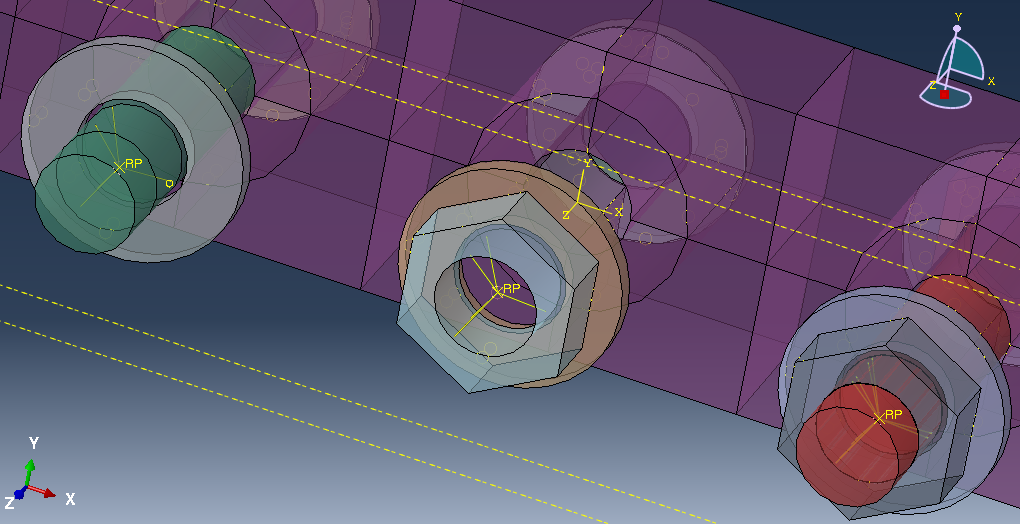
\includegraphics[width=0.55\textwidth]{./figs/conss.png}
\end{center}
\item We next create a static analysis step (\texttt{Step->Create Step->Static, General}) named as \texttt{PRESTRESS}.
This can be done in CAE, but here is the Python code.
\begin{verbatim}
51  mdl.StaticStep(name='PRESTRESS', previous='Initial', nlgeom=ON)
\end{verbatim}
\textbf{Note}: Nonlinear Geometric effects (nlgeom) is set to ON since this was found to be helpful for convergence of prestress analysis.
\item We finally apply bolt forces as concentrated forces at the \texttt{BPT-n} and \texttt{NPT-n} reference points.
Switch to the \texttt{Load} module to do this from CAE.
The following python code applies a tightening load of 12kN to each bolt.
\begin{verbatim}
52  # Apply forces
53  bpmag = 12e3  # 12kN bolt-load
54  for i in range(1, 4):
55      # Force in +z on bolt-points
56      mdl.ConcentratedForce(name='BoltLoad-%d' %(i), createStepName='PRESTRESS',
57                            region=ras.instances['BPT-%d' %(i)].sets['Set-1'],
58                            cf3=bpmag, distributionType=UNIFORM)
59  
60      # Force in -z on bolt-points
61      mdl.ConcentratedForce(name='NutLoad-%d' %(i), createStepName='PRESTRESS',
62                            region=ras.instances['NPT-%d' %(i)].sets['Set-1'],
63                            cf3=-bpmag, distributionType=UNIFORM)
\end{verbatim}
\begin{center}
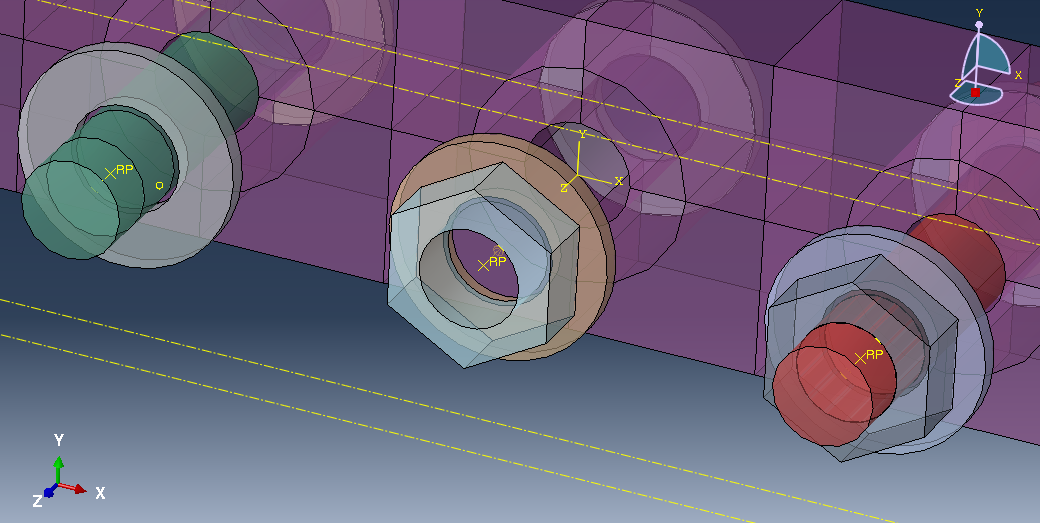
\includegraphics[width=0.55\textwidth]{./figs/loads.png}
\end{center}
\item \textbf{Note} that the bolt load constructed in the above manner is a "linear" load - i.e., the load can be increased/decreased by scaling the resulting force vector.
It is assumed here that all 3 bolts are loaded equally.
If this is not the case, the different loads can be exported separately and scaled appropriately (for external analysis).
It is, however, a physical requirement for equilibrium that \texttt{BoltLoad-n} and \texttt{NutLoad-n} have to be of equal magnitude and opposite signs.
\end{enumerate}

The file \href{https://github.com/Nidish96/Abaqus4Joints/blob/main/assets/assembly/model\_step1.cae}{model\_step1.cae} stores the CAE-file generated after the end of the above steps.
We will now proceed with meshing.
\section{Meshing}
\label{sec:org66acf12}
Since the model is perfectly symmetric, it is sufficient to mesh the model with a global seed, after seeding the interface area locally.
Switch to the \texttt{Mesh} module for this section.

If such symmetry is not available, one may choose a more direct approach by using the \texttt{bottom-up} meshing to copy the mesh from one interface to another directly.
Please \href{mailto:nidish.balaji@ila.uni-stuttgart.de}{write to me} if you'd like an example for this.
\subsection{Meshing Instructions\hfill{}\textsc{GUI}}
\label{sec:orga3134fd}
\begin{enumerate}
\item Choose \texttt{Mesh->Assign Mesh Controls} and select the whole assembly (all the instances).
We will use a structured hex-dominated element type for the full model (it will give a warning that this is not possible for certain regions. This is okay).
\begin{center}
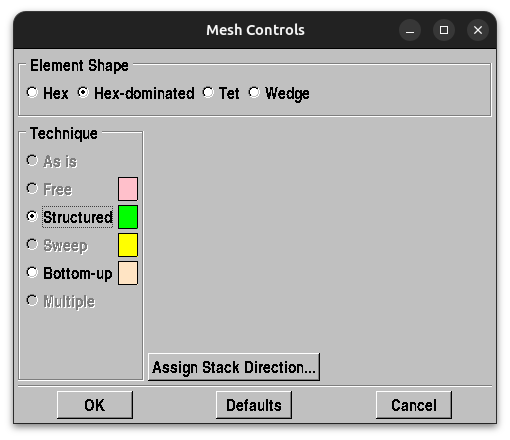
\includegraphics[width=0.5\textwidth]{./figs/globmesh.png}
\end{center}
\item Now choose \texttt{Mesh->Seed Part Instance} and select all the instances again.
Set 0.00254 as the global mesh seed (to ensure 10 elements across thickness) and 0.05 for curvature control.
\begin{center}
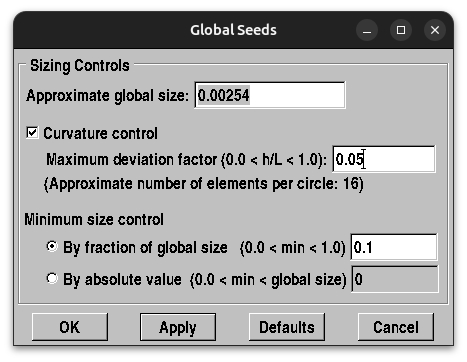
\includegraphics[width=0.5\textwidth]{./figs/gmeshseed.png}
\end{center}
\item Apply local seeds at the interface as shown here (on both interfaces).
Use the \texttt{Mesh->Seed Edges} tool by choosing the Method as "By Number" and specify the number of elements.
\begin{center}
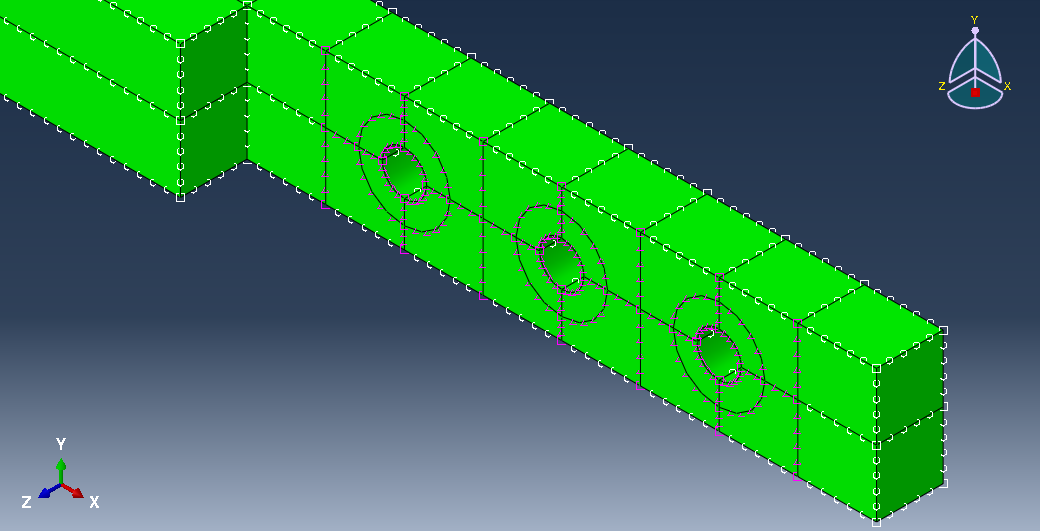
\includegraphics[width=0.55\textwidth]{./figs/lmeshseeds.png}
\end{center}
\item Now mesh the assembly using \texttt{Mesh->Mesh Part Instance} and selecting all the part instances.
Here is a view of the interfacial mesh you should get after the above seeding.
\begin{center}
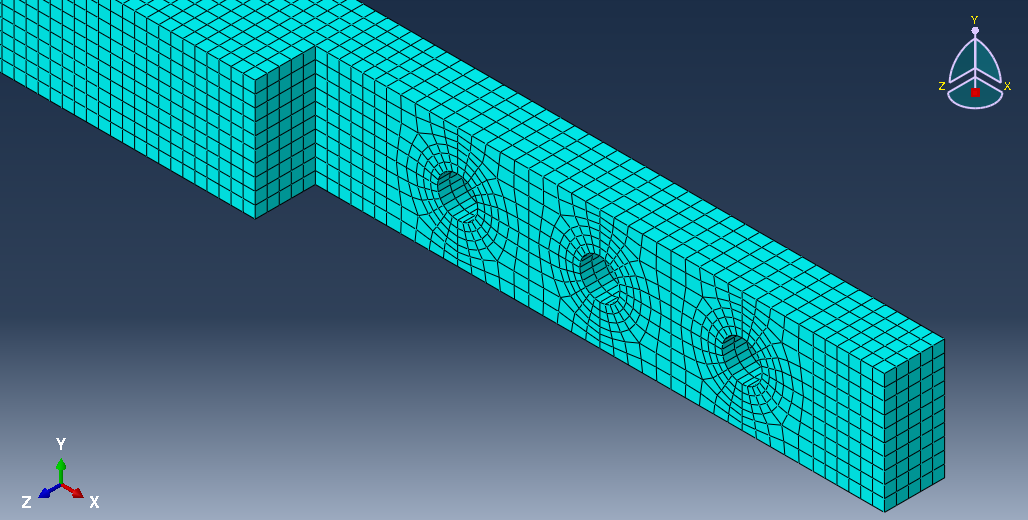
\includegraphics[width=0.5\textwidth]{./figs/mesh.png}
\end{center}
\item Here is an image of the total assembly with the mesh.
\begin{center}
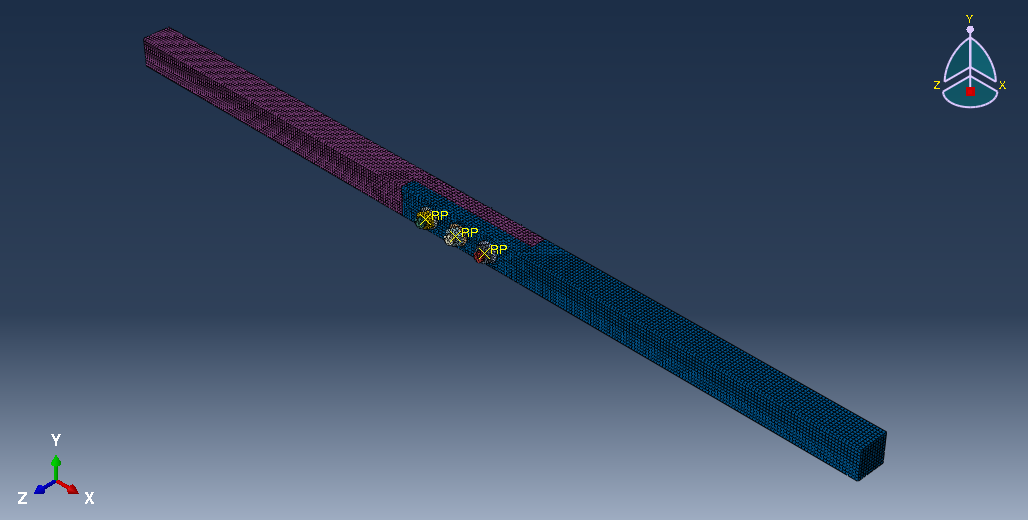
\includegraphics[width=0.55\textwidth]{./figs/fullmesh.png}
\end{center}
\end{enumerate}

The file \href{https://github.com/Nidish96/Abaqus4Joints/blob/main/assets/assembly/model\_step1.cae}{model\_step1.cae} stores the CAE-file along with the mesh.
\subsection{(Optional, recommended) Verify correctness of model through frictionless prestress\hfill{}\textsc{GUI}}
\label{sec:orgdd23dea}
We will now conduct a simple frictionless contact analysis to verify the correctness of the model.

\textbf{Setup}
\begin{enumerate}
\item For the static prestress analysis, first a surface-to-surface contact interaction property has to be created and assigned.
You can do this from CAE starting from \texttt{Interaction->Create Interaction} and following the steps in the figure below.
\begin{center}
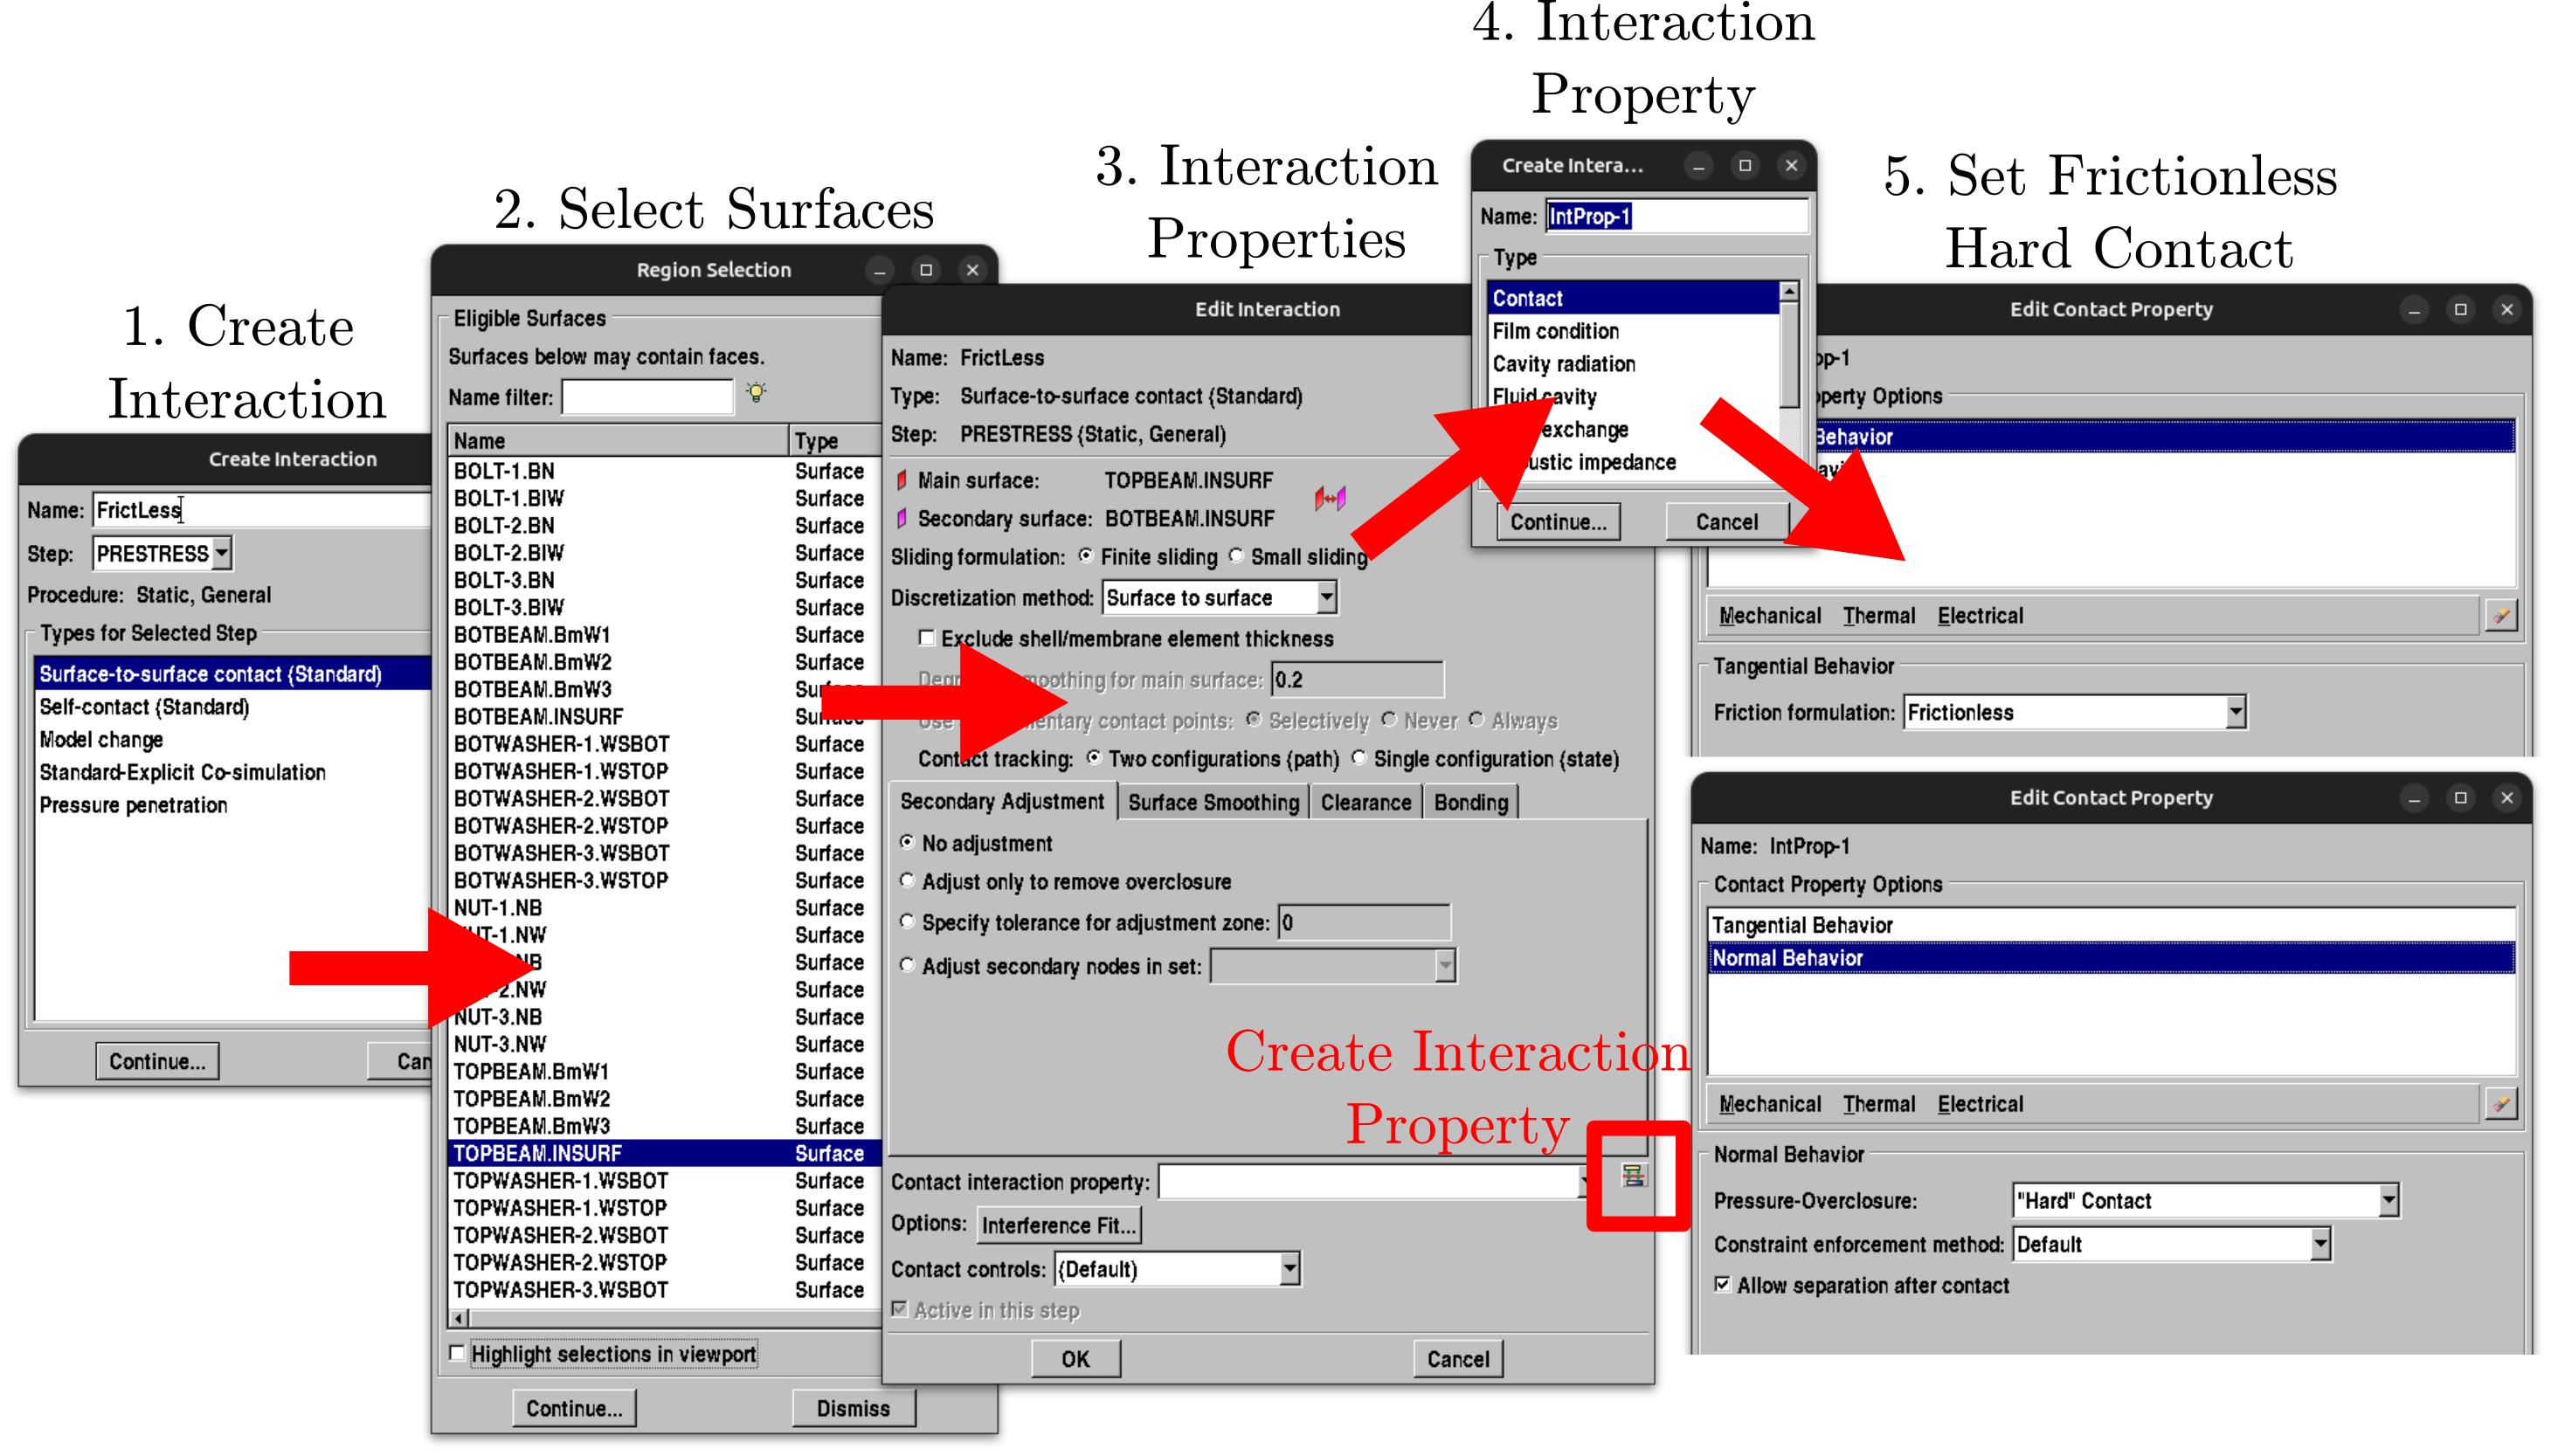
\includegraphics[width=.9\linewidth]{./figs/setcontact.png}
\end{center}
\item Now create two linear frequency steps, one before and one after the static prestress step, as shown in the figure below.
Request 30 eigenvalues in each case.
\begin{center}
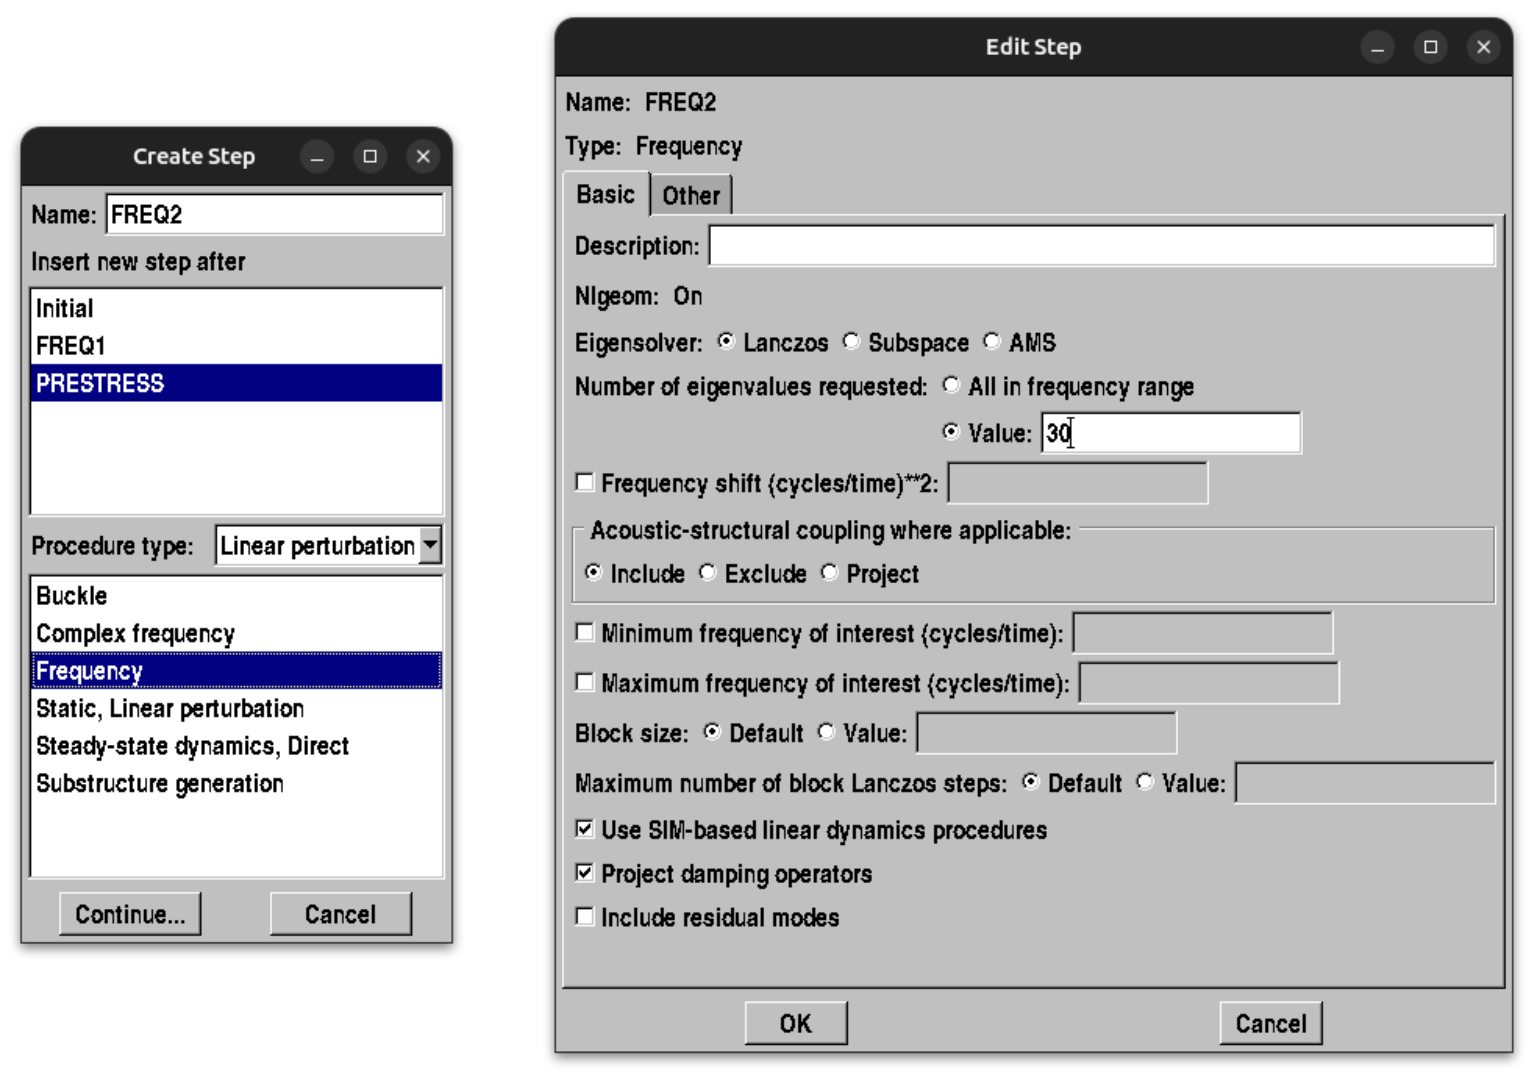
\includegraphics[width=0.55\textwidth]{./figs/lfreq.png}
\end{center}
\item Create 2 jobs. Suppress the interaction property in the first one and have just \texttt{FREQ1} active (see figure below).
\begin{center}
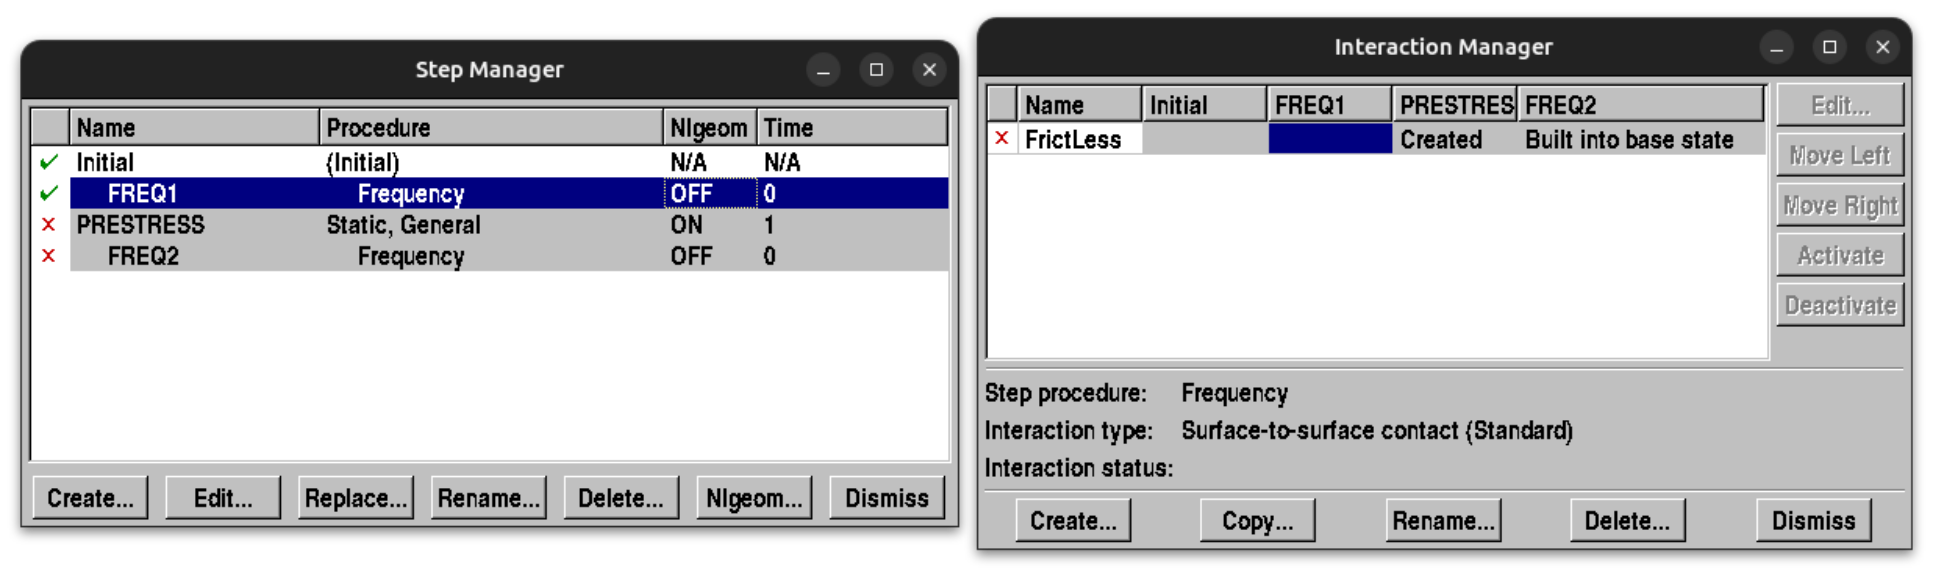
\includegraphics[width=.9\linewidth]{./figs/run1.png}
\end{center}
For the second job, suppress \texttt{FREQ1} and resume the other steps. Resume the surface interaction properties (see figure below).
\begin{center}
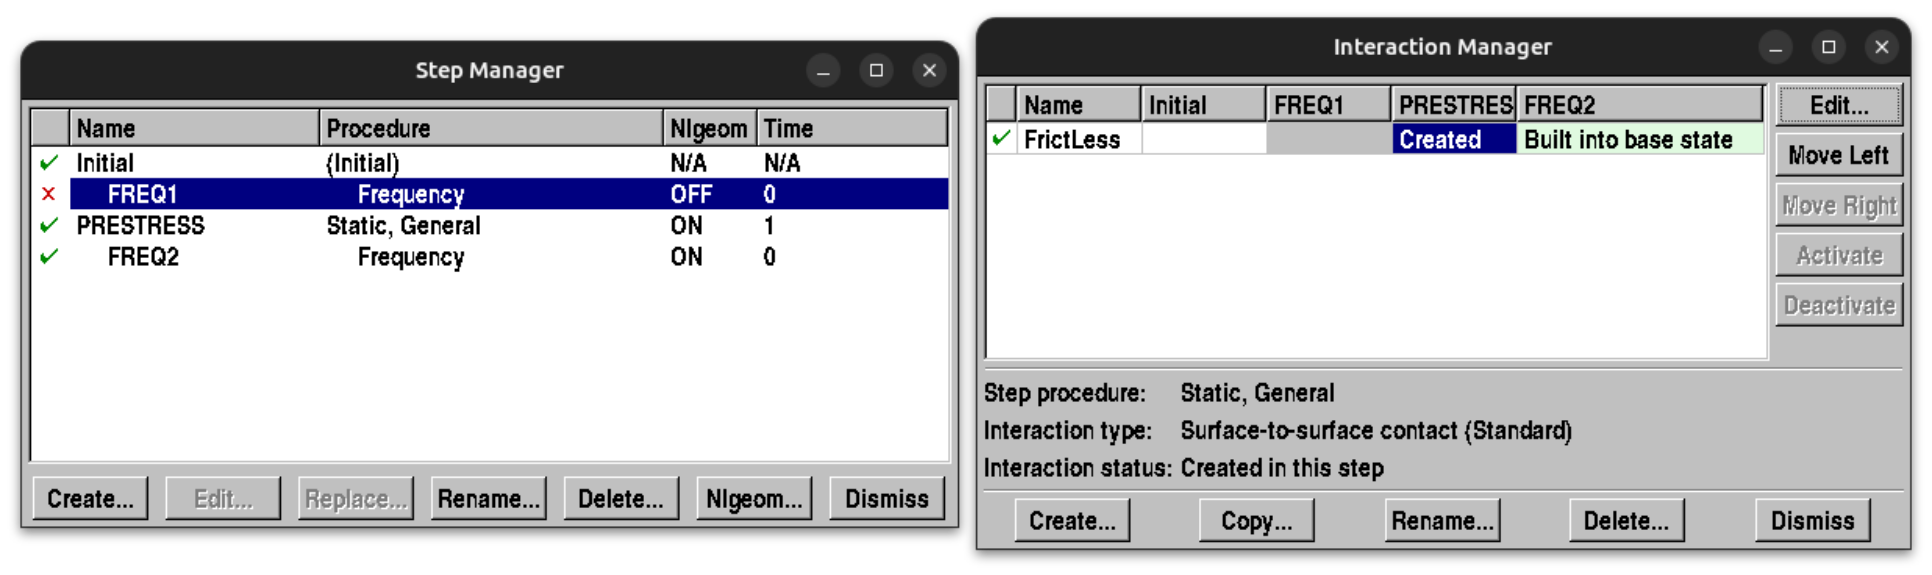
\includegraphics[width=.9\linewidth]{./figs/run2.png}
\end{center}
Optionally, field outputs for \texttt{FREQ2} (by default it will be set to none if \texttt{FREQ1} is suppressed).
You can do this in \texttt{Step->Create Field Outputs}.
\begin{center}
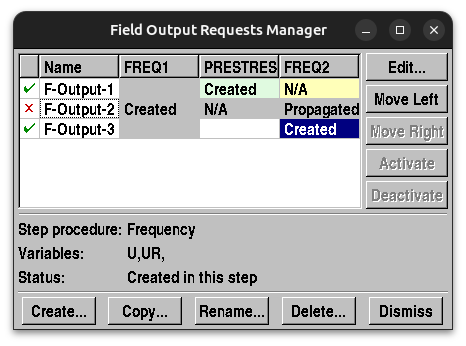
\includegraphics[width=0.5\textwidth]{./figs/run2_fo.png}
\end{center}
\end{enumerate}
\textbf{Results}
\begin{enumerate}
\item The first analysis should reveal that the system has \textbf{7 Rigid Body Modes} (RBMs).
This is because the two beams are  constrained together in all directions except the axial (where tightening has to happen).
So the number of RBMs has to be \(2\times 6 - 5 = 7\).
The first 10 modal frequencies have to be (frequencies in cycles/time, or Hz):
\begin{center}
\begin{tabular}{rr}
Index & Frequency\\[0pt]
\hline
1 & 1.0515e-3\\[0pt]
2 & 1.2851e-3\\[0pt]
3 & 1.4602e-3\\[0pt]
4 & 1.6246e-3\\[0pt]
5 & 1.6592e-3\\[0pt]
6 & 1.8082e-3\\[0pt]
7 & 1.9025e-3\\[0pt]
8 & 70.323\\[0pt]
9 & 151.26\\[0pt]
10 & 609.25\\[0pt]
\end{tabular}
\end{center}
In the above, modes 1-7 are RBMs and modes 8 onwards are the elastic modes.
Looking at the mode-shapes should make it clear that the two beams are free to move axially (the following is mode 1, for eg).
\begin{center}
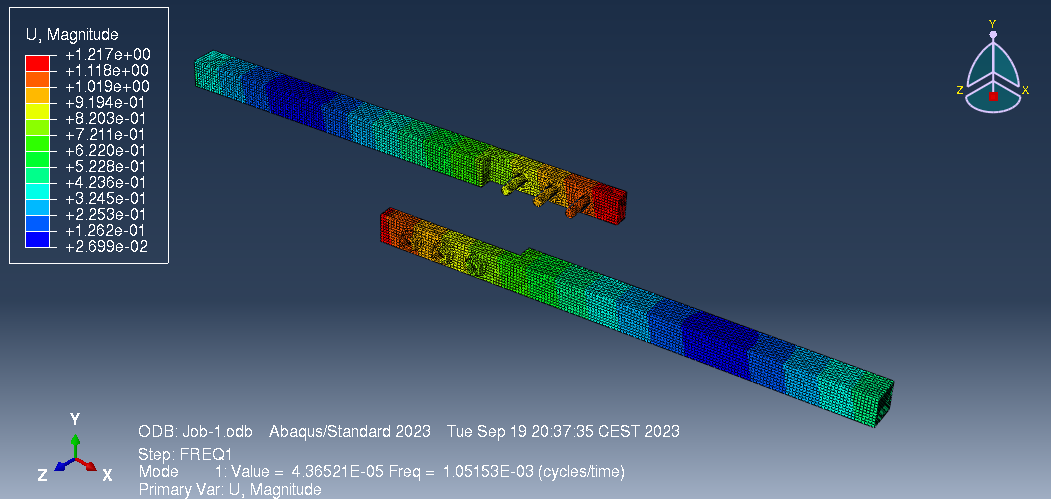
\includegraphics[width=0.55\textwidth]{./figs/res1.png}
\end{center}
\item The second analysis should converge within a few iterations.
If not, the "Initial Increment Size" in \texttt{Step->PRESTRESS->Edit->Increment->Initial Increment Size} has to be reduced.
If it doesn't converge, try to apply a boundary condition to make the problem well-posed, and try again.
If it still doesn't converge, check your model again.
Here is a picture of the contact pressures at the interface at the end of the static prestress step.
\begin{center}
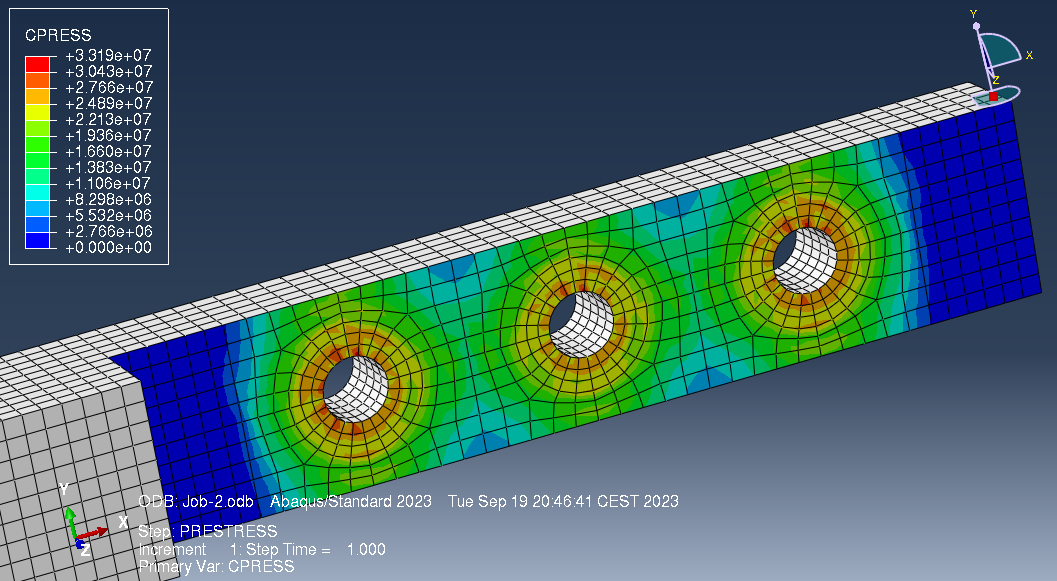
\includegraphics[width=0.55\textwidth]{./figs/res2_1.png}
\end{center}
\item By default, ABAQUS \textbf{fuses the nodes} that are in contact at the end of the hard contact step, for the eigenvalue analysis that follows it (Linear Perturbation step).
Since we are using frictionless tangential here, the tangential DOFs are not fused.
Here are the first 10 frequencies from the \texttt{FREQ2} step (frequencies in cycles/time, or Hz):
\begin{center}
\begin{tabular}{rr}
Index & Frequency\\[0pt]
\hline
1 & 0.00\\[0pt]
2 & 0.00\\[0pt]
3 & 0.00\\[0pt]
4 & 0.00\\[0pt]
5 & 0.00\\[0pt]
6 & 2.2068e-3\\[0pt]
7 & 141.10\\[0pt]
8 & 152.42\\[0pt]
9 & 570.33\\[0pt]
10 & 643.49\\[0pt]
\end{tabular}
\end{center}
It must be observed that the model, under the prestressed state, \textbf{has only 6 RBMs}.
In other words, the bolt-axial direction has now been fixed due to the fact that the contact constraints are active on at least one spot on the interface.
\item If your model passes all the above, then you are ready to proceed.
\textbf{INCLUDE NOTE ABOUT MESH CONVERGENCE?}
\end{enumerate}

The file \href{https://github.com/Nidish96/Abaqus4Joints/blob/main/assets/assembly/model\_step2.cae}{model\_step2.cae} is the cae file containing the model with the above tests included.
\section{Postprocessing}
\label{sec:org33b8fc0}
Now that the model is verified to be correct/consistent, we will proceed with the steps necessary for substructured Matrix Extraction.

Before proceeding it is necessary to first identify nodes on the meshed model that correspond to the input and output locations.
Choose the mid point on the right end as the output node for this tutorial.
Create a node set called \texttt{OutNodes} by selecting \texttt{Mesh->Tools->Set->Create->Node} and choosing the node. Select "unsorted node set" if available.
\begin{center}
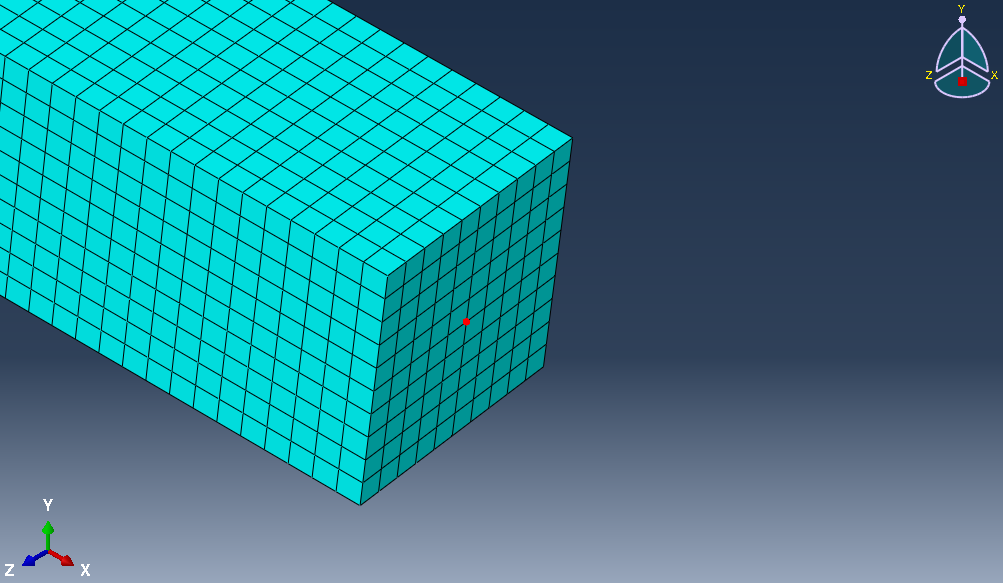
\includegraphics[width=0.5\textwidth]{./figs/outnode.png}
\end{center}
It is possible to choose multiple nodes here if you have a MIMO case.

It is also helpful to use global node and element indexing henceforth.
This can be specified in \texttt{Model->Edit Attributes->Model-1} as follows:
\begin{center}
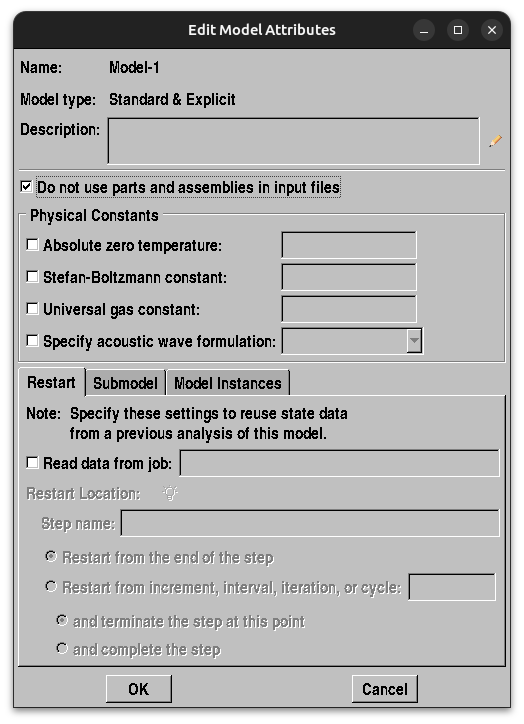
\includegraphics[width=0.5\textwidth]{./figs/modl.png}
\end{center}
\subsection{Reorganize Interfacial Node Sets (readjust if necessary)\hfill{}\textsc{Script}}
\label{sec:orgbcb1bc6}
Although we have taken care to ensure that the mesh of the \texttt{TOPBEAM} and \texttt{BOTBEAM} are conformal at the interface, minor imperfections in the nodal locations may exist.
Furthermore, the ordering of the nodes on the top interface will be different from that on the bottom interface.
Through some scripting, we can create node sets in such a way that the top and bottom interface nodesets are ordered in a convenient fashion.
\begin{enumerate}
\item We use the following slightly modified header for this script:
\begin{verbatim}
 1  # -*- coding: utf-8 -*-
 2  # 1. Preamble
 3  import sys
 4  import numpy as np
 5  
 6  from part import *
 7  from material import *
 8  from section import *
 9  from assembly import *
10  from step import *
11  from interaction import *
12  from load import *
13  from mesh import *
14  from optimization import *
15  from job import *
16  from sketch import *
17  from visualization import *
18  from connectorBehavior import *
19  
20  from abaqus import *
21  from abaqusConstants import *
22  from caeModules import * 
23  import regionToolset
24  import job
25  import step
26  import sets
27  
28  mdl = mdb.models['Model-1']
29  ras = mdl.rootAssembly
30  
31  mdl.setValues(noPartsInputFile=ON)
\end{verbatim}
\item Now we identify the top and bottom surface nodes, and store the top nodes and elements into separate variables.
The node and element ordering of the top nodes will be preserved, and the nodes in the bottom will be resorted according to this in \#3 below.
\begin{verbatim}
32  # 2. Get top and bottom surfaces and nodes
33  topsurf = ras.instances['TOPBEAM'].surfaces['INSURF']
34  botsurf = ras.instances['BOTBEAM'].surfaces['INSURF']
35  
36  topnodes = topsurf.nodes
37  botnodes = botsurf.nodes
38  N = len(topnodes)  # Number of nodes
39  
40  # Top Nodes and Coordinates
41  Topnd_dict = dict(zip([topnodes[i].label
42                         for i in range(N)], range(N)))
43  # maps original node ID (in FE model) to
44  # node ID in interface node set
45  TopNdCds = np.array([topnodes[i].coordinates
46                       for i in range(N)])
47  
48  # Top Elements
49  TopEls = np.array([topsurf.elements[i].connectivity
50                     for i in range(len(topsurf.elements))])
51  ELS = np.zeros((TopEls.shape[0], 5), dtype=int)
52  for ne in range(TopEls.shape[0]):
53      elefac = topsurf.elements[ne].getElemFaces()
54  
55      # Gives you the list of faces on the interface
56      # (we only expect a single face here)
57      fe = np.argwhere([all([Topnd_dict.has_key(x) for x in 
58                             [elefac[k].getNodes()[i].label
59                              for i in range(4)]])
60                        for k in range(6)])[0,0]
61      ELS[ne, 0] = ne
62      # Searches for the face where all the nodes are in the interface
63      # and returns those nodes
64      ELS[ne, 1:] = [Topnd_dict[x] for x in
65                     [elefac[fe].getNodes()[k].label
66                      for k in range(4)]]
67      ELS[ne, :] += 1
68  
69  # Save interfacial nodes and elements to txt files
70  np.savetxt('Nodes.dat', TopNdCds) # Save to dat file
71  np.savetxt('Elements.dat', ELS, fmt='%d')
\end{verbatim}
\item Now we extract the bottom nodes and sort them.
\begin{verbatim}
72  # 3. Node Pairing. We assume len(botnodes)=len(topnodes).
73  botleft = range(N)
74  bts = []
75  tmi = 0
76  for i in range(N):
77      # Calculates deviation of selected node coordinate on bottom to each
78      # node coordinate on top and "assigns" the closest one to the index.
79      devns = topnodes[i].coordinates - np.array([botnodes[j].coordinates
80                                                  for j in botleft])
81      bts.append(
82          botleft.pop(
83              np.argmin(
84                  np.linalg.norm(
85                      devns, axis=1)
86              )
87          )
88      )
\end{verbatim}
\item We now adjust the nodes on the bottom (this affects the FE mesh directly!)
\begin{verbatim}
89  # 4. Adjust Nodes on Bottom Beam Interface to Match Top Beam Exactly
90  for i in range(N):
91      ras.editNode(nodes=botnodes[bts[i]:bts[i]+1],
92                   coordinates=(topnodes[i].coordinates,))
\end{verbatim}
\item We now create nodesets for the top (\texttt{TOPS\_NDS}) and bottom (\texttt{BOTS\_NDS}).
\begin{verbatim}
 93  # 5. Create Node Sets
 94  botpairednds = botnodes.sequenceFromLabels(tuple([botnodes[i].label
 95                                                    for i in bts]))
 96  # Reordering from the sorting above
 97  
 98  ras.SetFromNodeLabels(name="TOPS_NDS", 
 99                        nodeLabels=((topnodes[0].instanceName, 
100                                     tuple([topnodes[i].label
101                                            for i in range(N)])),),
102                        unsorted=True)
103  ras.SetFromNodeLabels(name="BOTS_NDS", 
104                        nodeLabels=((botpairednds[0].instanceName, 
105                                     [botpairednds[i].label
106                                      for i in range(len(botpairednds))]),),
107                        unsorted=True)
\end{verbatim}
Note that we've used the unsorted keyword to ensure that ABAQUS does not reorder the nodesets (default behavior).
\item We now simplify the model by removing all interaction properties and steps (except initial).
One side-effect of doing this is that this removes the bolt loads also, since loads can only be saved when there is a corresponding step!
So we will reintroduce the bolt loads in the substructuring step in \#8 below.
\begin{verbatim}
108  # 6. Simplify model (remove interactions, all steps, etc.)
109  tmp = mdl.interactions
110  while len(tmp) > 0:
111      del tmp[tmp.keys()[-1]]
112  
113  tmp = mdl.interactionProperties
114  while len(tmp) > 0:
115      del tmp[tmp.keys()[-1]]
116  
117  # Remove all steps except initial
118  tmp = mdl.steps
119  while len(tmp) > 1:
120      del tmp[tmp.keys()[-1]]
\end{verbatim}
\end{enumerate}
\subsection{Setup Fixed interface CMS (HCB-CMS) with linear frequency and substructure steps\hfill{}\textsc{Script}}
\label{sec:org2bba903}
\begin{enumerate}
\item We are interested in \textbf{Fixed-Interface Component Mode Synthesis} with 20 retained modes.
So we first do a fixed interface modal analysis and request \(20\times3 = 60\) modes (for ensuring accuracy of the first 20 modes).
We fix all the nodes in the nodesets \texttt{TOPS\_NDS} and \texttt{BOTS\_NDS}.
\begin{verbatim}
121  # 7. Create a Frequency Step for fixed interface modal analysis
122  mdl.FrequencyStep(name="Fixed-Int-Modal", previous="Initial",
123                    normalization=MASS, eigensolver=LANCZOS,
124                    numEigen=60)
125  mdl.EncastreBC(name="TOPFIX", createStepName="Fixed-Int-Modal",
126                 region=ras.sets['TOPS_NDS'])
127  mdl.EncastreBC(name="BOTFIX", createStepName="Fixed-Int-Modal",
128                 region=ras.sets['BOTS_NDS'])
\end{verbatim}
\item Next, we create the substructuring step and re-specify the bolt loads (these were removed in \#6 above).
The bolt loads are specified of unit magnitude and can be scaled during analysis.
\textbf{This by default uses the mode shapes from the previous step and calculates static constraint modes automatically.}
\begin{verbatim}
129  # 8. Create a substructuring step, specify the modes and retained DOFs
130  mdl.SubstructureGenerateStep(name="HCBCMS", previous="Fixed-Int-Modal",
131                               substructureIdentifier=1, 
132                               retainedEigenmodesMethod=MODE_RANGE,
133                               modeRange=((1, 20, 1),),
134                               recoveryMatrix=REGION,
135                               recoveryRegion=ras.sets['OutNodes'],
136                               computeReducedMassMatrix=True)
137  
138  mdl.RetainedNodalDofsBC(name="TOPRET", createStepName="HCBCMS", 
139                          region=ras.sets['TOPS_NDS'], 
140                          u1=ON, u2=ON, u3=ON)
141  mdl.RetainedNodalDofsBC(name="BOTRET", createStepName="HCBCMS", 
142                          region=ras.sets['BOTS_NDS'], 
143                          u1=ON, u2=ON, u3=ON)
144  
145  # Apply Bolt Loads (1N magnitude)
146  for i in range(1, 4):
147      mdl.ConcentratedForce(name='BoltLoad-%d' %(i), createStepName="HCBCMS",
148                            cf3=1.0,
149                            region=ras.instances['BPT-%d' %(i)].sets['Set-1'])
150      mdl.ConcentratedForce(name='NutLoad-%d' %(i), createStepName="HCBCMS",
151                            cf3=-1.0,
152                            region=ras.instances['NPT-%d' %(i)].sets['Set-1'])
153  
154  sbs = mdl.steps['HCBCMS']
155  sbs.LoadCase(name="LCASE",
156               loads=tuple(('BoltLoad-%d' %(i), 1.0) for i in range(1, 4)) +
157               tuple(('NutLoad-%d' %(i), 1.0) for i in range(1, 4)))
\end{verbatim}
\item We finally need to request matrix output.
\href{https://classes.engineering.wustl.edu/2009/spring/mase5513/abaqus/docs/v6.6/books/key/default.htm?startat=ch18abk43.html}{Here} is the ABAQUS documentation for the \texttt{*Substructure Matrix Output} card.
Thus far (until version 2023) ABAQUS CAE doesn't support requesting matrix output from Substructure steps.
We have to request this manually in the .inp files.
Thankfully we can write to the keywords directly from CAE.
Go to \texttt{Model->Edit Keywords->Model-1} to do this in the GUI.
In scripting, this is known as a "synch" operation, which is done as follows:
\begin{verbatim}
158  # 9. Request substructure matrix outputs
159  # ABAQUS CAE doesn't support this yet (GUI or scripting),
160  # so the keywords need to be manually modified.
161  mdl.keywordBlock.synchVersions(storeNodesAndElements=False)
162  
163  li = np.argwhere([mdl.keywordBlock.sieBlocks[i][0:20] == "*Retained Nodal Dofs"
164                    for i in range(len(mdl.keywordBlock.sieBlocks))])[0][0]
165  txi = mdl.keywordBlock.sieBlocks[li]
166  mdl.keywordBlock.replace(li, "*Retained Nodal Dofs, sorted=NO"+txi[20:])
167  
168  mdl.keywordBlock.insert(len(mdl.keywordBlock.sieBlocks)-2, 
169                          "*Substructure Matrix Output, FILE NAME=Modelmats, " +
170                          "MASS=YES, STIFFNESS=YES, SLOAD=YES, " +
171                          "RECOVERY MATRIX=YES")
\end{verbatim}
\item We then create a job and write it to an "inp" file that can be run from ABAQUS.
\begin{verbatim}
172  # 10. Create a job and write an inp file
173  mdb.Job(name="Job", model='Model-1')
174  mdb.jobs['Job'].writeInput()
\end{verbatim}
\item Here is what the final HCBCMS step looks like in this case.
The most important part is the \texttt{*Substructure Matrix Output} card in the bottom,
which we introduced through the "synch" step in \#3 above.
\href{https://classes.engineering.wustl.edu/2009/spring/mase5513/abaqus/docs/v6.6/books/key/default.htm?startat=ch18abk43.html}{Here} is the ABAQUS documentation for the \texttt{*Substructure Matrix Output} card.
\begin{verbatim}
 1  ** ----------------------------------------------------------------
 2  ** 
 3  ** STEP: HCBCMS
 4  ** 
 5  *Step, name=HCBCMS, nlgeom=NO
 6  *Substructure Generate, overwrite, type=Z1, recovery matrix=YES,
 7        nset=OutNodes, mass matrix=YES
 8  *Select Eigenmodes, generate
 9  1, 20, 1
10  *Damping Controls, structural=COMBINED, viscous=COMBINED
11  *Retained Nodal Dofs, sorted=NO
12  BOTS_NDS, 1, 3
13  TOPS_NDS, 1, 3
14  ** 
15  ** LOAD CASES
16  ** 
17  *Substructure Load Case, name=LCASE
18  ** Name: BoltLoad-1   Type: Concentrated force   Scale factor: 1
19  *Cload
20  BPT-1_Set-1, 3, 1.
21  ** Name: BoltLoad-2   Type: Concentrated force   Scale factor: 1
22  *Cload
23  BPT-2_Set-1, 3, 1.
24  ** Name: BoltLoad-3   Type: Concentrated force   Scale factor: 1
25  *Cload
26  BPT-3_Set-1, 3, 1.
27  ** Name: NutLoad-1   Type: Concentrated force   Scale factor: 1
28  *Cload
29  NPT-1_Set-1, 3, -1.
30  ** Name: NutLoad-2   Type: Concentrated force   Scale factor: 1
31  *Cload
32  NPT-2_Set-1, 3, -1.
33  ** Name: NutLoad-3   Type: Concentrated force   Scale factor: 1
34  *Cload
35  NPT-3_Set-1, 3, -1.
36  *Substructure Matrix Output, FILE NAME=Modelmats, MASS=YES,
37        STIFFNESS=YES, SLOAD=YES, RECOVERY MATRIX=YES
38  *End Step
\end{verbatim}
\end{enumerate}
\subsection{Run Job and Generate the mtx file.\hfill{}\textsc{Script:GUI}}
\label{sec:orgdad92bb}
You can now run the Job named "Job" in the GUI, or directly run the "Job.inp" file from the command line using
\begin{verbatim}
abaqus job=Job inp=Job.inp cpus=2 interactive
\end{verbatim}
Once the job is done, it will output the matrix file "Modelmats.mtx" into the working directory.
This, along with the "Nodes.dat" and "Elements.dat" files that were written out earlier, are all we need for external analyses.
\section{Matrix Extraction}
\label{sec:orgeeecd8c}
By default, ABAQUS uses the \href{https://math.nist.gov/MatrixMarket/}{matrix market format} for the outputted matrices.
Note the following, in terms of format:
\begin{itemize}
\item Each line that starts with an asterix ("*") is a comment.
\item The linear matrices of the current model are fully symmetric.
\item So only the upper triangular parts of the matrices are exported.
\item The load vector is exported as a vector.
\item Columns of the recovery matrix \(R\), defined by
$$ x_{out} = R x_{cms} $$
where \(x_{cms}\) is the vector of DOFs of the CMS model (substructure) and \(x_{out}\) are the output DOFs.
Each column of \(R\) is \(N_{out}\times 1\), and \(R\) is \(N_{out}\times N_{cms}\).
\end{itemize}
\subsection{Postprocessing Exported Matrices\hfill{}\textsc{Script}}
\label{sec:orga970bdb}
\begin{enumerate}
\item The first few lines provide the generalized coordinates of the model. The nodes are listed as positive integers and the "modal" DOFs are listed as negative integers.
This is followed by a list of DOFs active in each set.
\item The STIFFNESS and MASS matrices are respectively prepended by
\begin{verbatim}
*     MATRIX,TYPE=STIFFNESS
      <Stiffness matrix entries in upper triangular form>

*     MATRIX,TYPE=MASS
      <Mass matrix entries in upper triangular form>      
\end{verbatim}
\item The load vector (the bolt prestress load, here) is written as,
\begin{verbatim}
** SUBSTRUCTURE LOAD CASE VECTOR. SLOAD CASE <name>
***CLOAD 
** 1, 1, <entry>
** 1, 2, <entry>
** 1, 3, <entry>
      .
      .
      .
\end{verbatim}
\item Finally, the recovery matrix is provided row-by-row as
\begin{verbatim}
*     SUBSTRUCTURE RECOVERY VECTOR CORRESPONDING TO RETAINED DOFS NUMBER 1
      <entries>
*     SUBSTRUCTURE RECOVERY VECTOR CORRESPONDING TO RETAINED DOFS NUMBER 2
      <entries>
      .
      .
      .
\end{verbatim}
\item In the actual file, the order is STIFFNESS, LOAD, MASS, then SUBSTRUCTURE.
\item The following Bash script processes the output (a stiffness, a mass, a load case, and recovery entries are expected)
\begin{verbatim}
  1  #!/bin/sh
  2  
  3  if [ $# = 2 ]
  4  then 
  5      echo "Correct call!"
  6      OUT=$2
  7  elif [ $# = 1 ]
  8  then
  9      echo "Acceptable call!"
 10      a="$1"
 11      OUT="${a%.*}.mat"
 12  else
 13      echo "Wrong call - quitting!"
 14  fi
 15  echo "Preprocessing mtx files"
 16  awkcmd1='BEGIN{mstart=0;}
 17    ($1~/^\*M/){mstart++; next}
 18    (mstart==1){if($1!~/^\*/){print}else{exit}}'
 19  awkcmd2='BEGIN{RS=",";ORS="\n"}{print}'
 20  gawk "$awkcmd1" $1|gawk "$awkcmd2"|gawk '(NF!=0){print}' > ./.STIFFNESS.mtx
 21  
 22  awkcmd1='BEGIN{mstart=0;}
 23    ($1~/^\*M/){mstart++; next}
 24    (mstart==2){if($1!~/^\*/){print}else{exit}}'
 25  awkcmd2='BEGIN{RS=",";ORS="\n"}{print}'
 26  gawk "$awkcmd1" $1|gawk "$awkcmd2"|gawk '(NF!=0){print}' > ./.MASS.mtx
 27  
 28  awkcmd1='BEGIN{vstart=0;}
 29    ($0~/^\*\*\*C/){vstart++; next}
 30    (vstart>0){print $2,$3,$4}
 31    (vstart>0 && $1!~/^\*\*/){exit}'
 32  awkcmd2='BEGIN{FS=","}
 33    {for(i=1;i<=NF;i++)
 34      printf("%s ", $i);
 35      printf("\n")}'
 36  gawk "$awkcmd1" $1|gawk "$awkcmd2" > ./.FVEC.mtx
 37  
 38  awkcmd1='BEGIN{rstart=0}
 39   ($0~/^\*\* SUBSTRUCTURE REC/){rstart++;
 40   if(rstart>1){printf("\n")}
 41   next}
 42   (rstart!=0 && $1~/\*\*/){
 43   for(i=2;i<=NF;i++)printf("%s",$i);}'
 44  awkcmd2='BEGIN{FS=","}
 45    {for(i=1;i<=NF;i++)
 46      printf("%s ",$i);
 47      printf("\n");}'
 48  gawk "$awkcmd1" $1|gawk "$awkcmd2" > .RECOV.mtx
 49  
 50  echo "Preprocessing mtx files done"
 51  
 52  python <<EOF
 53  import numpy as np
 54  import scipy.io as io
 55  
 56  print("Reading Mass Matrix from mtx file.");
 57  Mv = np.loadtxt('.MASS.mtx');
 58  print("Done.");
 59  
 60  print("Reading Stiffness Matrix from mtx file.");
 61  Kv = np.loadtxt('.STIFFNESS.mtx');
 62  print("Done.");
 63  
 64  print("Reading Recovery Matrix from mtx file.");
 65  R = np.loadtxt('.RECOV.mtx');
 66  print("Done.");
 67  
 68  print("Processing Matrices.")
 69  
 70  Nelm = len(Mv);
 71  Nelk = len(Kv);
 72  if (Nelm!=Nelk):
 73          sys.exit("GIGO - Mass & Stiffness not of same length.");
 74  Nel = Nelm;
 75  
 76  Nd = ((np.sqrt(1+8*Nel)-1)/2).astype(int); # Solution of Nd(Nd+1)/2-Nel = 0
 77  
 78  M = np.zeros((Nd,Nd));
 79  K = np.zeros((Nd,Nd));
 80  
 81  (xi,yi) = np.tril_indices(Nd);
 82  M[xi,yi] = Mv;
 83  M[yi,xi] = Mv;
 84  K[xi,yi] = Kv;
 85  K[yi,xi] = Kv;
 86  
 87  print("Done.")
 88  
 89  print("Reading Forcing Vector from mtx file.");
 90  Fvdat = np.loadtxt('.FVEC.mtx');
 91  print("Done.");
 92  
 93  print("Processing Force Vector.");
 94  Fv = np.zeros(M.shape[0]);
 95  ids = range(np.where(np.diff(Fvdat[:, 1])==0)[0][0], Fvdat.shape[0])
 96  n1dofnds = Fvdat[ids, 0].astype(int)
 97  n3dofnds = Fvdat[list(set(range(Fvdat.shape[0]))-set(ids)), 0].astype(int)
 98  Fv[((n3dofnds-1)*3+np.kron(np.ones(int(len(n3dofnds)/3)),[0, 1, 2])).astype(int)] = \
 99  Fvdat[list(set(range(Fvdat.shape[0]))-set(ids)), 2]
100  print("Whew.")
101  Fv[range(-len(n1dofnds), 0)] = Fvdat[ids, 2]
102  print("Done.")
103  
104  print("Matrix extraction complete - writing mat file")
105  dict = {"M": M, "K": K, "R": R.T, "Fv": Fv.reshape((len(Fv),1))};
106  io.savemat(".out.mat",dict);
107  print("Processing Over")
108  EOF
109  mv .out.mat $OUT
110  rm .STIFFNESS.mtx .MASS.mtx .RECOV.mtx .FVEC.mtx
\end{verbatim}
\begin{itemize}
\item This bash script first uses \href{https://www.gnu.org/software/gawk/manual/gawk.html}{GNU Awk}, a simple but powerful utility that allows line-by-line parsing of files.
\item The script also uses the \href{https://www.gnu.org/software/coreutils/cut}{cut} utility from \href{https://www.gnu.org/software/coreutils/cut}{GNU coreutils} for manipulations.
\item Finally, the script uses Python (compatible with 2/3), involving numpy and scipy.io, for converting the quantities into a MATLAB mat-file that can be loaded on MATLAB.
\item This script can be called as follows:
\begin{verbatim}
./readwritematvec.sh Modelmats.mtx
\end{verbatim}
\item In windows, this can be done either through \href{https://www.cygwin.com/}{Cygwin} or \href{https://learn.microsoft.com/en-us/windows/wsl/install}{Windows Subsystem for Linux}.
\end{itemize}
\item It may be possible to do this natively in MATLAB, but since this requires a line-parser, awk is better suited for the job than MATLAB.
A MATLAB implementation might require loading the whole file into memory for speed.
Line-parsing on MATLAB was extremely slow for me.
\end{enumerate}
The file \href{https://github.com/Nidish96/Abaqus4Joints/blob/main/assets/assembly/model\_step3.cae}{model\_step3.cae} is the final cae file that contains all of the above.
\subsection{Simple Analysis on MATLAB/OCTAVE\hfill{}\textsc{Script}}
\label{sec:org0364a6d}
We will now do our first nonlinear analysis on MATLAB/OCTAVE with the exported matrices.
We will conduct a \textbf{Nonlinear Prestress Analysis} for a frictionless contact with a unilateral spring on the normal direction.
\textbf{TO BE ADDED SOON}

\section{Outro/Contact Details}
\label{sec:org7e27041}
In summary, all the scripts used in the tutorial are provided in 
\begin{enumerate}
\item \href{https://github.com/Nidish96/Abaqus4Joints/blob/main/scripts/a\_steelmat.py}{a\_steelmat.py}: Loading material
\item \href{https://github.com/Nidish96/Abaqus4Joints/blob/main/scripts/b\_halfbm.py}{b\_halfbm.py}: Building the half-beam model
\item \href{https://github.com/Nidish96/Abaqus4Joints/blob/main/scripts/c\_nutwasherbolt\_516.py}{c\_nutwasherbolt\_516.py}: Building the bolt, nut, and washer models.
\item \href{https://github.com/Nidish96/Abaqus4Joints/blob/main/scripts/d\_applyconstraints.py}{d\_applyconstraints.py}: Applying the relevant constraints and introducing bolt prestress.
\item \href{https://github.com/Nidish96/Abaqus4Joints/blob/main/scripts/e\_nodeproc.py}{e\_nodeproc.py}: The postprocessing script create surface node sets and setting up substructure analysis.
\item \href{https://github.com/Nidish96/Abaqus4Joints/blob/main/scripts/readwritematvec.sh}{readwritematvec.sh}: Contains the mtx reading script written with \texttt{bash} and \texttt{python}.
\end{enumerate}

Don't forget to check out the repository in github at \href{https://github.com/Nidish96/Abaqus4Joints}{https://github.com/Nidish96/Abaqus4Joints}.
It has the above scripts as well as all the cae files.

You can contact me at \href{mailto:nidish.balaji@ila.uni-stuttgart.de}{nidish.balaji@ila.uni-stuttgart.de} or \href{mailto:nidbid@gmail.com}{nidbid@gmail.com} for any questions/suggestions.
\end{document}